%======================================================================
%   Zak Webb
%   Ph.D. Thesis
%   Department of Physics and Astronomy
%   University of Waterloo
% 
%   Universality of multi-particle scattering
%======================================================================


\documentclass[../thesis-main/thesis-main]{subfiles}
\begin{document}

\chapter{Universality of multi-particle scattering}


\todo{I should really give a broad overview of the technique.  Maybe not in any great detail, but I should really explain why things are going to go the way they are.}

In the previous chapter, we were able to show that the single-particle scattering on a large enough graph allowed for universal quantum computation.  However, the graph had a number of vertices exponential in the number of simulated qubits.  While the evolution was still time efficient, the underlying graph had to be a graph in the Hilbert space as opposed to an actual implementable graph.

To get around this, we need to somehow enlarge the Hilbert space while keeping the number of vertices of the graph small.  If we use a vertex for each basis vector of the Hilbert space, we will not be able to shrink the graph down to any reasonable size.  However, if we instead use some correlations in addition to the graph structure in order to encode computations we can reduce the size of the graph.

In particular, if we use multiple particles as opposed to a single particle, the resulting Hilbert space grows like $V^N$, where $V$ is the number of vertices and $N$ is the number of particles.  Hence, if we encode computation using a number of particles that grows like the number of simulated qubits, we can keep the size of the underlying graph small.

The main ideas of this chapter follow \cite{MPQW}, with various improvements from \cite{MomSwitches}.  However, the proof of \thm{two_particle_wavepacket_bound}, while inspired by proofs in \cite{MPQW} is novel to this thesis.

\todo{a lot more citations}

\section{Multi-particle quantum walk}

We have already seen how a single particle moves on some given graph; the evolution proceeds with the Hamiltonian given by the adjacency matrix of the graph.  If we want to extend this framework to multiple particles, we should ensure that each particle still has this single-particle evolution.

Namely, if we assume that $N$ particles each move independently on a given graph $G$, we will want the Hamiltonian of this larger system to be as though each particle sees its own copy of $G$.  To do this, we will have that the $N$ particle quantum walk with no interaction takes the form
\begin{align}
  H_{\text{mov}}^N = \sum_{w\in [N]} A(G)^{(w)}
\end{align}
where $B^{(w)}$ is the operator that acts on $N$ particles as $B$ on the $w$th particle and $\II$ on the rest, or
\begin{align}
  B^{(w)} = \II_{|V(G)|}^{\otimes w-1} \otimes B \otimes \II_{|V(G)|}^{N - w}.
\end{align}
With such a Hamiltonian, the evolution operator decomposes into a product of commuting terms, where each term acts as the single particle evolution for a different particle.  This is exactly what we would want for the $N$-particle case.

However, the eigenstates of such a Hamiltonian are simply product states over the $N$ particles, where each of the particles are an eigenstate of $A(G)$.  Such a system is only as computationally powerful as that of a single-particle, since the individual particles cannot interact.  As such, for our purposes we will want to include some interaction.  We also want to ensure that we capture the intuitive structure of particle interactions in the continuum, where the interaction only depends on the distance between particles.  This translation invariance can have several different abstractions to a general graph, but on a one dimensional lattice we would expect the interaction to only depend on the distance between the particles, as measured by the shortest path between vertices.

We will take this requirement on the infinite path and use it for all vertices.  Futher, we will assume some finite range of interaction, so that particles with large physical separation don't interact.   Namely, let us choose some $\dmax \in \NN$ to be the finite range of the interaction, and then choose $d+1$ symmetric polynomials in two variables, $U_{d}$ for $0\leq d \leq \dmax$.  Additionally, let $\hat{n}_v$ for $v\in V(G)$ be the operator that counts the number of particles at vertex $v$, explicitly given by 
\begin{align}
  \hat{n}_v = \sum_{w\in [N]} \ketbra{v}{v}^{(w)}.
\end{align}
With these values, and if $d(u,v)$ is the distance function on the graph $G$ given by the length of the shortest path between $u$ and $v$, we can define the interaction
\begin{align}
  H_{\text{int}} = \sum_{d=0}^{\dmax} \sum_{\substack{ u,v\in V(G)\\d(u,v) = d}}U_{d} (\hat{n}_u,\hat{n}_v).
\end{align}
Note that on the infinite path (and in fact on any lattice), this interaction has the form we require.

With such a chosen interaction, (i.e., with $\dmax$ and the $U_d$ well defined), we can then define the $N$-particle quantum walk on $G$ with this interaction.  Namely, we let 
\begin{align}
  H_G^N = H_{\text{mov}}^N + H_{\text{int}}^N = \sum_{w\in [N]} A(G)^{(w)} + \sum_{d=0}^{\dmax}  \sum_{\substack{ u,v\in V(G)\\d(u,v) = d}}U_{d} (\hat{n}_u,\hat{n}_v). 
  \label{eq:MPQW_H_defn}
\end{align}
Hamiltonians of this form will be the study of this thesis.


As a particular example, if $\dmax = 0$, and 
\begin{align}
  U(x,y) = \gamma \frac{x + y}{4} (x + y -2)
\end{align}
we have an onsite interaction with strength $\gamma$, for which, if we restrict our attention to symmetric states, is the Bose-Hubbard Hamiltonian with strength $\frac{\gamma}{2}$.  Similarly, if $\dmax = 0$, $U_0 (x,y) = 0$ and $U_1(x,y) = \gamma xy$, we have a nearest-neighbor interaction with strength $\gamma$.




\section{Two-particle scattering on an infinite path}

With our chosen interactions, we now have a well defined $N$-particle quantum walk.  However, we have very few analytic solutions to any problems with these Hamiltonians (as this is the purpose of this thesis).  As such, we will attempt to understand these Hamiltonians in highly restricted systems, hoping that the results for these smaller systems will allow us to understand the $N$-particle states.

Since we already have an understanding of single-particle scattering, the next most simple case will be two-particle interactions on an infinite path.  Let us assume that the interaction Hamiltonian has been chosen, such that there is a $\dmax$ and a set of functions $U_d$.  We can then write the Hamiltonian \eq{MPQW_H_defn} in the basis $\ket{x,y}$, where $x,y\in \ZZ$ are the positions of the first and second particles, as
\begin{align}
  H^{2} = H^1_{x} \otimes \II_y + \II_x \otimes H^1_y + \sum_{x\in \ZZ} \sum_{d=0}^{\dmax} U_{d} (\hat{n}_x,\hat{n}_{x+d}) ,
  \label{eq:two_part_H}
\end{align}
where the single-particle Hamiltonian $H^1$ is simply the adjacency matrix for the infinite path, namely
\begin{align}
  H^{1} = \sum_{x\in\ZZ} \ket{x+1}\bra{x} + \ket{x}\bra{x+1}.
\end{align}

Without the interaction term, the eigenstates for this Hamiltonian would simply by two independent scattering eigenstates, with amplitudes of the form $e^{i k x + i py}$.  However, the interaction causes there to be correlations between the two particles.  These correlations will be similar to the single particle interactions scattering off of a graph with two attached semi-infinite paths.

As we are interested in the dynamics of two particles initially prepared in spatially separated wave packets moving toward each other along the path with momenta $k_1\in(-\pi,0) $ and $k_2\in (0,\pi)$, we will need to understand these scattering eigenstates.

\subsection{Scattering Eigenstates}

Attempting to use the symmetry of these Hamiltonians to our advantage, we will derive scattering eigenstates of this Hamiltonian by transforming to the new variables $s = x+y$ and $r = x-y$.  Here the allowed values $(s,r)$ range over the pairs of integers where either both are even or both are odd.  Writing states in this basis as $|s;r\rangle$, the Hamiltonian \eq{two_part_H} takes the form
\begin{equation}
  H^{(1)}_s\otimes H^{(1)}_r+ \II_s\otimes \sum_{r\in \ZZ} \mathcal{V}(|r|) \, \ket{r}\bra{r},
\label{eq:twopart_ham}
\end{equation}
where $V(0) = U_0(2,2)$ and $V(r) = U_r(1,1)$ for $r >0$.  For each $p_1\in (-\pi,\pi)$ and $p_2\in(0,\pi)$ there is a scattering eigenstate $|\mathrm{sc}(p_1;p_2)\rangle$ of the form
\begin{align}
\langle s;r |\mathrm{sc}(p_1;p_2)\rangle=e^{-ip_1 s/2} \langle r|\psi(p_1;p_2)\rangle,
\end{align}
where the state $|\psi(p_1;p_2)\rangle$ can be viewed as an effective single-particle scattering state of the Hamiltonian
\begin{equation}
 2\cos\left(\frac{p_1}{2}\right) H^{(1)}_r + \sum_{r\in \ZZ} \mathcal{V}(|r|) \, \ket{r}\bra{r}\label{eq:vr_eqn}
\end{equation}
with eigenvalue $4 \cos( p_1/2) \cos(p_2)$.  For a given $\mathcal{V}$, this is simply a single-particle scattering problem as described in \chap{scattering_on_graphs}, although the interior graph $\widehat{G}$ might be weighted.  As such, we have that the state $\ket{\psi(p_1;p_2)}$ can be written as
\begin{equation}
\langle r|\psi (p_1;p_2)\rangle= \begin{cases}  e^{-i p_2 r} + R(p_1,p_2) e^{i p_2 r} &  \text{if } r \leq -\dmax\\
  	f(p_1,p_2,r) &  \text{if } |r| < \dmax\\
  	T(p_1,p_2) e^{- i p_2 r}  & \text{if } r \geq \dmax\end{cases}
\label{eq:psip1p2}
\end{equation}
for $p_2\in (0,\pi)$. Here the reflection and transmission coefficients $R$ and $T$ and the amplitudes of the scattering state for $|r|<\dmax$ (described by the function $f$) depend on both momenta as well as the interaction $\mathcal{V}$.  With $R$, $T$, and $f$ chosen appropriately, the state $|\mathrm{sc}(p_1;p_2)\rangle$ is an eigenstate of $H^{(2)}$ with eigenvalue $4\cos(p_1/2)\cos(p_2)$.

\todo{if I want to give a better error bound, I'll need to talk about the dimer states}

Since $\mathcal{V}(|r|)$ is an even function of $r$, we can also define scattering states for $p_2\in (-\pi,0)$ by
\begin{align}
\langle s;r|\mathrm{sc}(p_1;p_2)\rangle=\langle s;-r|\mathrm{sc}(p_1;-p_2)\rangle.
\end{align}
These other states are obtained by swapping $x$ and $y$, corresponding to interchanging the two particles.

\todo{double check this}	
The construction of the symmetric and anti-symmetric scattering states follows as one would expect. For $p_1\in (-\pi,\pi)$ and $p_2\in (0,\pi)$, we define
\begin{align}
  \ket{\mathrm{sc}(p_1;p_2)}_\pm = \frac{1}{\sqrt2}\big(\ket{\mathrm{sc}(p_1;p_2)} \pm \ket{\mathrm{sc}(p_1;-p_2)}\big).
\end{align}
If we note that the unitarity of $S$ and the fact that $V(|r|)$ being even in $r$ forces $R(p_1,p_2) = R(p_1,-p_2)$ and $T(p_1,p_2)  = T(p_1,-p_2)$ we can then see that the combinations
\begin{align}
  |T(p_1,p_2) \pm R(p_1,p_2)| = 1.  
\end{align}
With this, we can then see that the symmeterized scattering states can be expanded as
\begin{align}
    \braket{s;r}{\mathrm{sc}(p_1;p_2)}_\pm
      &= \frac{1}{\sqrt{2}}e^{-i p_1 s/2} \begin{cases}  e^{i p_2 |r|} \pm e^{i\theta_{\pm}(p_1,p_2)} e^{-i p_2 |r|} &  \text{if } |r| \geq C\\
  	f(p_1,p_2,r) \pm f(p_1,p_2,-r) & \text{if }  |r| < C\end{cases}
\label{eq:symscatter}
\end{align}
where $\theta_{\pm}(p_1,p_2)$ is a real function defined through
\begin{equation}
e^{i\theta_{\pm}(p_1,p_2)}= T(p_1,p_2)\pm R(p_1,p_2). \label{eq:delta_pm}
\end{equation}


These eigenstates allow us to understand what happens when two particles with momenta $k_1\in(-\pi,0)$ and $k_2\in(0,\pi)$ move toward each other. Here $p_1=-k_1-k_2$ and $p_2=(k_2-k_1)/2$.  Similar to the scattering states of \chap{scattering_on_graphs}, we have that for $|r|\geq C$ the scattering state is a sum of two terms, one corresponding to the two particles moving toward each other and one corresponding to the two particles moving apart after scattering, but where the outgoing term has a  phase of $T\pm R$ relative to the incoming term (as depicted in \fig{wte}). This phase arises from the interaction between the two particles.



\begin{figure}
  \centering
  \tikzsetnextfilename{MP_u_wte}
  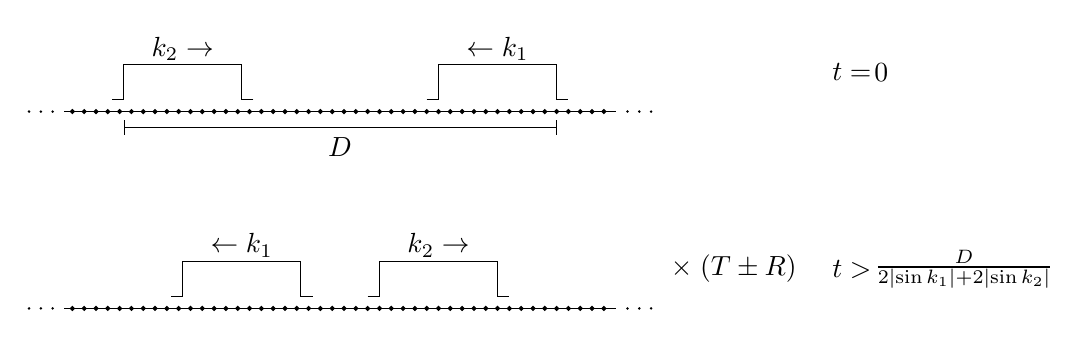
\begin{tikzpicture}[label distance= -6pt,
    verts/.style={circle,draw=black,fill=black,inner sep=.5pt,minimum size=0pt},
    dots/.style={circle,fill=black,inner sep=.25pt,minimum width=0pt}]
  \draw (0,0) -- (7,0);

  
  \draw (3.15,.15) -- (3,.15) -- (3,.6) -- (1.5,.6) 
     -- (1.5,.15) -- (1.35,.15);
  
  \draw (3.85,.15) -- (4,.15) -- (4,.6) -- (5.5,.6) 
     -- (5.5,.15) -- (5.65,.15);
     
  \node at (2.25,.8) {$\leftarrow k_1$};
  \node at (4.75,.8) {$k_2\rightarrow$};

  \node at (8.5,.5) {$\times \; (T\pm R)$};

  \node at (10,.5)[label=right:$\frac{D}{2|{\sin k_1}|+ 2|{\sin k_2}|}$]{$t>$};
  

  \foreach \x in {.1,.25,...,6.9}
  \node at (\x ,0) [verts] {};
  
  \begin{scope}[yshift=2.5cm]
    \draw (0,0) -- (7,0);

    \draw[xshift=-.75cm] (3.15,.15) -- (3,.15) -- (3,.6) -- (1.5,.6) 
       -- (1.5,.15) -- (1.35,.15);
  
    \draw[xshift=.75cm] (3.85,.15) -- (4,.15) -- (4,.6) -- (5.5,.6) 
       -- (5.5,.15) -- (5.65,.15);
 
    \draw [|-|] (.75,-.2) to node[below] {$D$} (6.25,-.2);
    
    \node at (1.5,.8) {$k_2\rightarrow$};
    \node at (5.5,.8) {$\leftarrow k_1$};

    \node at (10,.5)[label=right:$0$] {$t=$};

    \foreach \x in {.1,.25,...,6.9}
    \node at (\x ,0) [verts] {};

  \end{scope}

  \foreach \xsh in {-0.45cm, 7.15cm}{
  \foreach \ysh in {0cm, 2.5cm}{
    \begin{scope}[xshift=\xsh,yshift=\ysh]
      \node at (0,0) [dots]{};
      \node at (0.15,0) [dots] {};
      \node at (0.3,0) [dots]{};
    \end{scope}
  }}

\end{tikzpicture}
  \caption{Scattering of two particles on an infinite path.}
  \label{fig:wte}
\end{figure}


\subsection{Examples}

\todo{I don't like this section here.  Find a place to put it}

For example, consider the Bose-Hubbard model, where $\mathcal{V}(|r|) = U\delta_{r,0}$. Here $C=0$ and $T=1+R$.  In this case the scattering state $|\mathrm{sc}(p_1;p_2)\rangle_+$ is
\begin{align}
\langle x,y|\mathrm{sc}(p_1;p_2)\rangle_+=\frac{1}{\sqrt{2}}e^{-ip_1 \left(\frac{x+y}{2}\right)}\left(e^{ip_2 |x-y|}+e^{i\theta_+(p_1,p_2)}e^{-ip_2 |x-y|}\right).
\end{align}
The first term describes the two particles moving toward each other and the second term describes them moving away from each other. To solve for the applied phase $e^{i\theta_+(p_1,p_2)}$ we look at the eigenvalue equation for $|\psi(p_1;p_2)\rangle$ at $r=0$. This gives
\begin{align}
  R(p_1,p_2) =- \frac{U}{U - 4i\cos({p_1}/{2})\sin(p_2)}.
\end{align}
So for the Bose-Hubbard model,
\begin{align}
  e^{i \theta_{+} (p_1,p_2)} = T(p_1,p_2) + R(p_1,p_2) = - \frac{ U + 4 i \cos({p_1}/{2}) \sin(p_2)}{U - 4 i \cos({p_1}/{2}) \sin(p_2)} =  \frac{2 \left(\sin(k_2) - \sin(k_1)\right) - i U}{2 \left(\sin(k_2) - \sin(k_1)\right) + i U}.
\end{align}
For example, if $U = 2+\sqrt{2}$ then two particles with momenta $k_1 =-{ \pi}/{2}$ and $k_2={\pi}/{4}$ acquire a phase of $e^{-i\pi/2}= -i$ after scattering.

For a multi-particle quantum walk with nearest-neighbor interactions, $\mathcal{V}(|r|)=U\delta_{|r|,1}$ and $C=1$.  In this case the eigenvalue equations for $|\psi(p_1;p_2)\rangle$ at $r=-1$, $r=1$, and $r=0$ are
\begin{align*}
 4 \cos\left(\frac{p_1}{2}\right)  \cos(p_2) ( e^{i p_2} + R(p_1,p_2) e^{-i p_2} ) &= U ( e^{i p_2} + R(p_1,p_2) e^{-i p_2}) \\
& \quad + 2\cos\left(\frac{p_1}{2}\right) \left( e^{2i p_2} + R(p_1,p_2) e^{-2i p_2}+f(p_1,p_2,0)\right) \\
 4 \cos\left(\frac{p_1}{2}\right)  \cos(p_2) T(p_1,p_2) e^{-ip_2} & =UT(p_1,p_2)e^{-ip_2}\\
& \quad +2\cos \left(\frac{p_1}{2}\right)\left(f(p_1,p_2,0)+T(p_1,p_2)e^{-2ip_2}\right)\\
2 \cos(p_2) f(p_1,p_2,0) &=T(p_1,p_2)e^{-ip_2}+e^{ip_2}+R(p_1,p_2)e^{-ip_2},
\end{align*}
respectively.

Solving these equations for $R$, $T$, and $f(p_1,p_2,0)$, we can construct the corresponding scattering states for bosons, fermions, or distinguishable particles (for more on the last case, see \sec{distinguishable}). Unlike the case of the Bose-Hubbard model, we may not have $1+R=T$. For example, when $U=-2-\sqrt{2}$, $p_1={\pi}/{4}$, and $p_2={3\pi}/{8}$, we get $R=0$ and $T=i$ (see \sec{distinguishable}).

\subsection{Two-particle basis}

\todo{Can I bootstrap Andrew and David's basis result to decompose the identity?}


The states $\{|\mathrm{sc}(p_1;p_2)\rangle \colon p_1\in (-\pi,\pi),\,p_2\in(-\pi,0)\cup(0,\pi)\}$ are (delta-function) orthonormal:
\begin{align*}
\langle  \mathrm{sc}(p_1';p_2')|\mathrm{sc}(p_1;p_2)\rangle &= \langle \mathrm{sc}(p_1'; p_2')|\left(\sum_{\text{$r,s$ even}}|r\rangle\langle r| \otimes |s\rangle \langle s| \right)|\mathrm{sc}(p_1;p_2)\rangle\\
&\quad + \langle \mathrm{sc}(p_1'; p_2')|\left(\sum_{\text{$r,s$ odd}}|r\rangle \langle r|\otimes  |s\rangle \langle s|\right)|\mathrm{sc}(p_1;p_2)\rangle\\
&= \sum_{\text{$s$ even}} e^{-i(p_1-p_1') {s}/{2}}\sum_{\text{$r$ even}}\langle \psi(p_1';p_2')|r\rangle\langle r|\psi(p_1;p_2)\rangle \\
& \quad + \sum_{\text{$s$ odd}} e^{-i(p_1-p_1') {s}/{2}}\sum_{\text{$r$ odd}}\langle  \psi(p_1';p_2')|r\rangle\langle r|\psi(p_1;p_2)\rangle\\
&= 2\pi \delta(p_1-p_1') \sum_{r=-\infty}^{\infty}\langle \psi(p_1;p_2')|r\rangle\langle r|\psi(p_1;p_2)\rangle\\
&= 4\pi^2 \delta(p_1-p_1')\delta(p_2-p_2')
\end{align*}
where in the last step we used the fact that $\langle\psi(p_1;p_2')|\psi(p_1;p_2)\rangle=2\pi\delta(p_2-p_2')$.


%%%%%%%%%%%%%%%%%
%  Finite Truncation

\subsection{Wavepacket Scattering}

\todo{go over section, ensure correct, and make equations all fit}

Now that we have a thorough understanding of the two-particle scattering eigenstates on an infinite path, we will want to understand the time-evolution of wavepackets on the infinite path.  In particular, if we initially have a product state corresponding to two Guassian wavepackets traveling towards each other, how does the time-evolved state look?

Along those lines, let $k\in(-\pi,\pi)$, and let $\mu \in \NN$.  We will define a Gaussian wavepacket centered at $\mu$, with momentum $k$, standard deviation $\sigma$, and cutoff $L$ as the state
\begin{align}
  \ket{\chi_{\mu,k}} = \gamma \sum_{x=\mu-L}^{\mu+L} e^{i k x} e^{ -\frac{(x-\mu)^2}{2\sigma^2}} \ket{x},
\end{align}
where $\gamma^2$ is a normalization factor given by $\gamma^{-2} = h_L^{\sigma/\sqrt{2}}(0)$.  Note that this is nearly the same state as for single-particle scattering, but now we don't have to deal with the multiple semi-infinite paths and the graph $\widehat{G}$.

This section is focused on proving the following lemma discussing wavepacket propagation:
%%%%%%%%%%%%%%%%%%%%%%%%%%%%%%%%%%%
\begin{theorem}
Let $H^{(2)}$ be a two-particle Hamiltonian of the form \eq{something} with interaction range at most $C$.  Let $\theta_{\pm}(p_1,p_2)$ be given by equation \eq{something_else}.  Let $k_1\in (-\pi,0)$ and let $k_2 \in (0,\pi)$, let $L,\mu, \nu \in \NN$ with $L>0$ and $\mu < \nu - 2 L$, and let $\sigma > 0$.  Let us then define the states
\begin{align}
  \ket{\psi(0)}_{\pm} = \frac{1}{\sqrt{2}} \big( \ket{\chi_{\mu, k_1}} \ket{\chi_{\nu, k_2}} \pm  \ket{\chi_{\nu,k_2}}\ket{\chi_{\mu,k_1}}\big),
\end{align}
and 
\begin{align}
  &\ket{\alpha (t)}_{\pm} \nonumber\\
  &\qquad= \frac{e^{-2 i t (\cos(k_1) + \cos(k_2))}}{\sqrt{2}} 
    e^{i \theta_{\pm}(t)} \big( \ket{\chi_{\mu(t),k_1}}\ket{\chi_{\nu(t),k_2}}  \pm \ket{\chi_{\nu(t),k_2}}\ket{\chi_{\mu(t),k_1}}\big) ,
\end{align}
where
\begin{align}
  \mu(t) = \mu - \lceil 2 t \sin k_1\rceil, \quad
  \nu(t) = \nu - \lceil 2 t \sin k_2\rceil, \quad \text{and} \quad 
  \theta_{\pm}(t)=\begin{cases}0 & t < \frac{ \nu - \mu - 2 L}{2 \sin k_2 - 2\sin k_1}\\
  \theta_{\pm}(k_1,k_2)& t > \frac{\nu - \mu + 2 L}{2 \sin k_2 - 2 \sin k_1}.\end{cases}
\end{align}
If $\sigma = \frac{ L}{2\sqrt{\log L}}$, and if $0 \leq t < \frac{ \nu - \mu - 2 L}{2 \sin k_2 - 2\sin k_1}$ or if $\frac{\nu - \mu + 2L}{2 \sin k_2 - 2\sin k_1}< t < c L$ for some constant $c$, then 
\begin{align}
  \norm{e^{ - i H^2 t} \ket{\psi(0)}_{\pm} - \ket{\alpha(t)}}_{\pm} \leq \chi_2 \sqrt{\frac{\log L}{L}}
\end{align}
for some constant $\chi_2$.
\label{thm:two_particle_wavepacket_bound}
\end{theorem}

Note that we will use many of the tools used in the proof of \thm{single_particle_wavepacket_bound}.

\begin{proof}
The main idea behind this proof will be to show that $\ket{\psi(0)}$ and $\ket{\alpha (t)}$ are both well approximated by a Gaussian distribution over eigenstates of $H^{(2)}$ with momenta near $k_1$ and $k_2$, and then show that time evolving the Gaussian approximation for $\ket{\psi(0)}$ is well approximated by the Gaussian approximation for $\ket{\alpha(t)}$.  
  
In particular, let us examine the inner product between an eigenstate $\ket{\scat (p_1;p_2)}_{\pm}$ and $\ket{\alpha(t)}_{\pm}$.  Note that $\ket{\scat(p_1;p_2)}_{\pm}$ has no overlap with $\ket{\alpha(t)}_{\mp}$, and 
\begin{align}
  &{}_{\pm}\braket{\scat(p_1;p_2)}{\alpha(t)}_\pm \nonumber\\
  & \qquad= \frac{e^{-2 i  t (\cos(k_1) + \cos(k_2)) + i\theta_{\pm}(t)}}{\sqrt{2}} \big({}_{\pm}\braket{\scat (p_1;p_2)}{\chi_{\mu(t),k_1},\chi_{\nu(t),k_2}}  \pm {}_{\pm}\braket{\scat(p_1;p_2)}{\chi_{\nu(t),k_2},\chi_{\mu(t),k_1}}\big).
\end{align}
We will then want to investigate the overlap between $\ket{\scat(p_1;p_2)}$ and the cut-off Gaussian approximations.  In particular, if we assume that $s - r > 2 L$, then 
\begin{align}
   &_{\pm}\braket{\scat(p_1;p_2)}{\chi_{r,k_1},\chi_{s,k_2}}\nonumber\\
    &\qquad= \gamma^2\sum_{x=r-L}^{r+L} \sum_{y=s-L}^{L} e^{ik_1x}e^{-\frac{(x-r)^2}{2\sigma^2}} e^{i k_2 y}e^{-\frac{(y-s)^2}{2\sigma^2}} \braket{\scat(p_1;p_2)}{x,y}\\
   &\qquad= \gamma^2\sum_{x=r-L}^{r+L} \sum_{y=s-L}^{s+L} e^{i (k_1 x + k_2 y)} e^{-\frac{(x-r)^2 + (y-s)^2}{2\sigma^2}} \frac{e^{i p_1 \frac{x+y}{2}}}{\sqrt{2}} \Big( e^{  i p_2 | x - y|} \pm e^{-i\theta_{\pm}(p_1,p_2) - i p_2 |x-y|}\Big)\\
   &\qquad = \gamma^2\frac{e^{i (k_1 r + k_2 s + p_1 \frac{r+s}{2} + p_2 (s - r))}}{\sqrt{2}} \sum_{x=-L}^{L} \sum_{y=-L}^L e^{ -\frac{ x^2 + y^2}{2\sigma^2}}e^{i ( k_1 + \frac{p_1}{2} -p_2) x} e^{i (k_2 + \frac{p_1}{2} + p_2)y} \nonumber\\
   &\qquad \qquad + \gamma^2 \frac{e^{i (k_1 r + k_2 s + p_1 \frac{r+s}{2} + p_2 (r-s) - i \theta_\pm(p_1,p_2))}}{\sqrt{2}} \sum_{x=-L}^{L} \sum_{y=-L}^L e^{ -\frac{ x^2 + y^2}{2\sigma^2}}e^{i ( k_1 + \frac{p_1}{2} +p_2) x} e^{i (k_2 + \frac{p_1}{2} - p_2)y}\\
   &\qquad = \gamma^2\frac{e^{i (k_1 + \frac{p_1}{2} - p_2) r + i (k_2 + \frac{p_1}{2} + p_2)s}}{\sqrt{2}} h_L^\sigma\bigg( k_1 + \frac{p_1}{2} - p_2\bigg) h_{L}^\sigma \bigg(k_2 + \frac{p_1}{2} + p_2\bigg)\nonumber\\
   &\qquad \qquad +\gamma^2 \frac{e^{i (k_1 + \frac{p_1}{2} + p_2) r + i (k_2 + \frac{p_1}{2} - p_2)s - i\theta_{\pm}(p_1,p_2)}}{\sqrt{2}} h_L^\sigma\bigg( k_1 + \frac{p_1}{2} + p_2\bigg) h_{L}^\sigma \bigg(k_2 + \frac{p_1}{2} - p_2\bigg).
\end{align}
If $s - r < -2L$, then nearly the same argument holds, and we find
\begin{align}
   &_{\pm}\braket{\scat(p_1;p_2)}{\chi_{r,k_1},\chi_{s,k_2}}\nonumber\\
   &\qquad = \gamma^2 \frac{e^{i (k_1 + \frac{p_1}{2} + p_2) r + i (k_2 + \frac{p_1}{2} - p_2)s}}{\sqrt{2}} h_L^\sigma\bigg( k_1 + \frac{p_1}{2} + p_2\bigg) h_{L}^\sigma \bigg(k_2 + \frac{p_1}{2} - p_2\bigg)\nonumber\\
   &\qquad \qquad +\gamma^2\frac{e^{i (k_1 + \frac{p_1}{2} - p_2) r + i (k_2 + \frac{p_1}{2} + p_2)s - i\theta_{\pm}(p_1,p_2)}}{\sqrt{2}} h_L^\sigma\bigg( k_1 + \frac{p_1}{2} - p_2\bigg) h_{L}^\sigma \bigg(k_2 + \frac{p_1}{2} + p_2\bigg).
\end{align}
Putting these bounds together, if we define $p_1 = -(k_1 + k_2)$ and $2 p_2 = k_1 - k_2$, we find that for $t < \frac{\nu - \mu - 2L}{2 \sin k_2 - 2 \sin k_1}$
\begin{align}
  &{}_{\pm}\braket{\scat(p_1 + \phi_1 ; p_2 + \phi_2)}{\alpha(t)}_{\pm} \nonumber\\
  &\qquad    = \gamma^2e^{-2 i  t (\cos(k_1) + \cos(k_2))} e^{i \phi_1\frac{\mu(t) + \nu(t)}{2}} \Bigg[e^{i \phi_2 (\nu(t) - \mu(t)) } h_{L}^\sigma \bigg(\frac{\phi_1}{2} - \phi_2\bigg) h_L^\sigma\bigg( \frac{\phi_1}{2} + \phi_2\bigg)\nonumber\\
  &\qquad\qquad \pm e^{ i (2 p_2+\phi_2)(\mu(t) - \nu(t)) - i \theta_{\pm}(p_1 + \phi_1, p_2+\phi_2)}h_L^\sigma\bigg(\frac{\phi_1}{2} - 2p_2 - \phi_2 \bigg) h_L^\sigma\bigg(\frac{\phi_1}{2} + 2 p_2 + \phi_2\bigg)\Bigg].
\end{align}
In nearly the same manner, if $ t > \frac{\nu - \mu + 2 L}{2 \sin k_2 - 2 \sin k_1}$, we have
\begin{align}
  &{}_{\pm}\braket{\scat(p_1 + \phi_1 ; p_2 + \phi_2)}{\alpha(t)}_{\pm} \nonumber\\
  &\qquad    = \gamma^2e^{-2 i  t (\cos(k_1) + \cos(k_2)) + i \theta_{\pm}(p_1,p_2)} e^{i\phi_1\frac{\mu(t) + \nu(t)}{2}} \Bigg[e^{i \phi_2 (\nu(t) - \mu(t)) - i \theta_{\pm}(p_1 + \phi_1, p_2+\phi_2) } h_{L}^\sigma \bigg(\frac{\phi_1}{2} - \phi_2\bigg) h_L^\sigma\bigg( \frac{\phi_1}{2} + \phi_2\bigg)\nonumber\\
  &\qquad\qquad \pm e^{ i (2 p_2+\phi_2)(\mu(t) - \nu(t)) }h_L^\sigma\bigg(\frac{\phi_1}{2} - 2p_2 - \phi_2 \bigg) h_L^\sigma\bigg(\frac{\phi_1}{2} + 2 p_2 + \phi_2\bigg)\Bigg].
\end{align}

With these useful inner products, we can now define our Gaussian approximations.  In particular, we will define the states
\begin{align}
  \ket{w(t)} &= \eta e^{ - 2 i t (\cos k_1 + \cos k_2)} \int_{-\delta}^\delta \int_{-\delta}^\delta \frac{d\phi_1 d\phi_2}{4\pi^2} e^{i \phi_1 \big(\frac{\mu(t) + \nu(t)}{2}\big)} e^{i  \phi_2 (\nu(t) - \mu(t))} e^{ -\frac{ \sigma^2 \phi_1^2}{4}} e^{ -\sigma^2 \phi_2^2} \ket{\scat(p_1 + \phi_1; p_2 + \phi_2)}_{\pm}
\end{align} 
where
\begin{align}
  \eta^{-2} &= \int_{-\infty}^\infty \int_{-\infty}^\infty \frac{d\phi_1 d\phi_2}{4\pi^2} e^{ -\sigma^2 \big(\frac{\phi_1^2}{2} + 2 \phi_2^2 \big)} = \frac{1}{4\pi\sigma^2}.
\end{align}
While the states $\ket{w(t)}$ are not exactly normalized, we have that
\begin{align}
   \braket{w(t)}{w(t)} &= \eta^2 \int_{-\delta}^\delta \int_{-\delta}^\delta \frac{d\phi_1d\phi_2}{4\pi^2}  e^{ -\sigma^2 \big(\frac{\phi_1^2}{2} + 2 \phi_2^2 \big)} &= 1  - \frac{\eta^2}{\pi^2} \int_\delta^{\infty} \int_{\delta}^\infty d\phi_1d\phi_2 e^{ - \sigma^2 \big(\frac{\phi_1^2}{2} + 2 \phi_2^2\big)}\\
   & \geq  1 - \frac{1}{\pi \delta^2 \sigma^2}e^{- \frac{5 \sigma^2 \delta^2}{2}},
\end{align}
and as the second term on the right hand side is non-negative, we have that $\braket{w(t)}{w(t)} \leq 1$.

As in the single-particle case, we will want to show that the overlap between $\ket{w}$ and $\ket{\alpha(t)}_\pm$ is nearly 1.  In particular, for $0 \leq t < \frac{\nu(t) - \mu(t) - 2 L}{2 \sin k_2 - 2 \sin k_1}$, we then have that
\begin{align}
  &\braket{w(t)}{\alpha(t)}_\pm \nonumber\\
  &\qquad= \eta \gamma^2  \int_{-\delta}^\delta \int_{-\delta}^\delta \frac{d\phi_1 d \phi_2}{4\pi^2}  e^{-\frac{\sigma^2 \phi_1^2}{4}}  e^{- \sigma^2 \phi_2^2}\Big[h_L^\sigma \big(\frac{\phi_1}{2} - \phi_2 \big) h_L^\sigma\Big( \frac{\phi_1}{2} + \phi_2 \Big) \nonumber\\
  & \qquad \quad\pm e^{ i \theta_{\pm}(p_1+\phi_1, p_2+\phi_2)} e^{ 2 i( p_2 + \phi_2)(\mu(t) - \nu(t))} h_L^\sigma\Big(\frac{\phi_1}{2} - 2 p_2 - \phi_2\Big) h_L^\sigma\Big(\frac{\phi_1}{2}+ 2 p_2 + \phi_2\Big)\Big]\\
  & \qquad = \eta\gamma^2 \int_{-\delta}^\delta \int_{-\delta}^\delta \frac{d\phi_1 d\phi_2}{4\pi^2} e^{- \frac{\sigma^2 \phi_1^2}{4}}e^{-\sigma^2 \phi_2^2} \Bigg[ h_\infty^\sigma(\frac{\phi_1}{2} - \phi_{2} ) h_{\infty}^\sigma ( \frac{\phi_1}{2} + \phi_2) \nonumber\\
  &\qquad\quad 
   + \Big[h_L^{\sigma} \Big(\frac{\phi_1}{2} + \phi_2 \Big)  + h_\infty^\sigma \Big(\frac{\phi_1}{2} + \phi_2 \Big)\Big] \Big[ h_{L}^\sigma\Big(\frac{\phi_1}{2} - \phi_2 \Big) - h_\infty^\sigma\Big(\frac{\phi_1}{2} - \phi_2\Big)\Big]\nonumber\\
   &\qquad \quad\pm e^{ i \theta_{\pm}(p_1+\phi_1, p_2+\phi_2)} e^{ 2 i( p_2 + \phi_2)(\mu(t) - \nu(t))}  \Big[h_L^{\sigma} \Big(\frac{\phi_1}{2} + 2p_2 +\phi_2 \Big)  + h_\infty^\sigma \Big(\frac{\phi_1}{2} + 2p_2+ \phi_2 \Big)\Big] \nonumber\\
   &\qquad \quad \qquad \times\Big[ h_{L}^\sigma\Big(\frac{\phi_1}{2} -2p_2 - \phi_2 \Big) - h_\infty^\sigma\Big(\frac{\phi_1}{2} -2p_2- \phi_2\Big)\Big]\nonumber\\
   &\qquad \quad\pm e^{ i \theta_{\pm}(p_1+\phi_1, p_2+\phi_2)} e^{ 2 i( p_2 + \phi_2)(\mu(t) - \nu(t))}h_\infty^{\sigma} \Big(\frac{\phi_1}{2} + 2p_2 +\phi_2 \Big) h_\infty^{\sigma} \Big(\frac{\phi_1}{2} - 2p_2 -\phi_2 \Big) \Bigg].
\end{align}
While this expression looks rather complicated, most of the amplitude is a result of the first term in the integrand, and the rest of the terms are simply small error terms resulting from approximating $h_L^\sigma$ by $h_\infty^\sigma$ or cross terms between the pre- and post-scattering amplitudes.  As such, we will bound each term individually, giving upper and lower bounds on the first term, and only upper bounds on the norm of the latter terms.

For the first term, we have
\begin{align}
  &\int_{-\delta}^\delta \int_{-\delta}^{\delta} \frac{ d\phi_1 d\phi_2}{4\pi^2} e^{ - \frac{\sigma^2\phi_1^2}{4} - \sigma^2 \phi_2^2} h_\infty^\sigma \Big(\frac{\phi_1}{2} - \phi_2\Big) h_\infty^\sigma \Big( \frac{\phi_1}{2} + \phi_2\Big)\nonumber\\
  & \qquad =  \frac{\sigma^2}{2\pi} \int_{-\delta}^\delta \int_{-\delta}^\delta d\phi_1 d\phi_2 e^{ -\frac{\sigma^2 \phi_1^2}{2} - 2\sigma^2 \phi_2^2} h_\infty^{1/(2\pi \sigma)} \Big[2 \pi i \sigma^2 \Big(\frac{\phi_1}{2} - \phi_2 \Big)\Big]h_\infty^{1/(2\pi \sigma)} \Big[2 \pi i \sigma^2 \Big(\frac{\phi_1}{2} +\phi_2 \Big)\Big]\\
 & \qquad \geq \frac{\sigma^2}{2\pi} \int_{-\delta}^\delta \int_{-\delta}^\delta d\phi_1 d\phi_2 e^{ -\frac{\sigma^2 \phi_1^2}{2} - 2\sigma^2 \phi_2^2}\\
 & \qquad = \frac{1}{2} \braket{w(t)}{w(t)}
\end{align}
where we used the fact that $h_\infty^\sigma(i \phi) \geq 1$.  Using the upper bounds on $h$, we also have that
\begin{align}
&\int_{-\delta}^\delta \int_{-\delta}^{\delta} \frac{ d\phi_1 d\phi_2}{4\pi^2} e^{ - \frac{\sigma^2\phi_1^2}{4} - \sigma^2 \phi_2^2} h_\infty^\sigma \Big(\frac{\phi_1}{2} - \phi_2\Big) h_\infty^\sigma \Big( \frac{\phi_1}{2} + \phi_2\Big)\nonumber\\
& \qquad \leq \frac{\sigma^2}{2\pi} \int_{-\delta}^\delta \int_{-\delta}^\delta d\phi_1 d\phi_2 e^{ -\frac{\sigma^2 \phi_1^2}{2} - 2\sigma^2 \phi_2^2} \Bigg[1 + 2 \Big(1 + \frac{ 1}{\pi \sigma^2} \frac{1}{4 \pi -  | \phi_1 - 2\phi_2|} \Big)e^{-2\pi^2 \sigma^2 + \pi \sigma^2 (\phi_1 - 2 \phi_2)} \Bigg]\nonumber\\
& \qquad \qquad \times   \Bigg[1 + 2 \Big(1 + \frac{ 1}{\pi \sigma^2} \frac{1}{4 \pi -  | \phi_1+ 2\phi_2|} \ \Big)e^{-2\pi^2 \sigma^2 +   \pi \sigma^2 (\phi_1 + 2 \phi_2)} \Bigg]\\
& \qquad \leq \frac{1}{2} \Big[1 + 3 e^{ -  \pi^2 \sigma^2 \big(2 \pi - 3\delta\big)} \Big]^2  \braket{w(t)}{w(t)}
\end{align}
where we assumed that $2\pi > 3 \delta$, and that $\sigma \geq 1$. 

For the second term, note that for any $\varphi_1$, $\varphi_2$, and for any $L > \sigma \geq 1$, we have that
\begin{align}
  &\big| \big(h_L^\sigma(\varphi_1) + h_{\infty}^\sigma(\varphi_1)\big)\big(h_L^\sigma(\varphi_2) - h_\infty^\sigma(\varphi_2) \big) \big| \nonumber\\
  &\qquad\leq \big| h_L^\sigma(\varphi_1) + h_{\infty}^\sigma(\varphi_1)\big| \frac{2\sigma^2}{L} e^{-\frac{L^2}{2\sigma^2}}\\
   & \qquad\leq \frac{2 \sigma^2}{L} e^{-\frac{L^2}{2\sigma^2} }\Big [ 2 + \big|h_L^\sigma (\varphi_2) - h_\infty^\sigma(\varphi_2) \big| + 2 \big| 1 - h_\infty^\sigma(\varphi_2) \big| \Big]\\
   & \qquad \leq  \frac{2 \sigma^2}{L} e^{-\frac{L^2}{2\sigma^2} }\Big [ 2 +   \frac{2 \sigma^2}{L} e^{-\frac{L^2}{2\sigma^2} }  + 4 (1 + \sigma^2) e^{ -\frac{1}{2\sigma^2}}\Big]\\
   & \qquad \leq \frac{24 \sigma^4}{L}  e^{ - \frac{L^2}{2\sigma^2}}.
\end{align}
If we then use this bound for the integrand, we have 
\begin{align}
  &\Bigg | \int_{-\delta}^\delta \int_{-\delta}^\delta \frac{d\phi_1 d\phi_2}{4\pi^2} e^{- \frac{\sigma^2 \phi_1^2}{4}}e^{-\sigma^2 \phi_2^2}  \Big[h_L^{\sigma} \Big(\frac{\phi_1}{2} + \phi_2 \Big)  + h_\infty^\sigma \Big(\frac{\phi_1}{2} + \phi_2 \Big)\Big] \Big[ h_{L}^\sigma\Big(\frac{\phi_1}{2} - \phi_2 \Big) - h_\infty^\sigma\Big(\frac{\phi_1}{2} - \phi_2\Big)\Big]\Bigg|\nonumber\\
  & \qquad \leq  \int_{-\delta}^\delta \int_{-\delta}^\delta \frac{d\phi_1 d\phi_2}{4\pi^2} e^{- \frac{\sigma^2 \phi_1^2}{4}}e^{-\sigma^2 \phi_2^2}  \frac{24 \sigma^4}{L}  e^{-\frac{L^2}{2\sigma^2}}\\
  & \qquad \leq \frac{6\sigma^4}{\pi^2 L}  e^{ - \frac{ L^2}{2\sigma^2}}\int_{-\infty}^\infty \int_{-\infty}^\infty  d\phi_1 d\phi_2 e^{- \frac{\sigma^2 \phi_1^2}{4}}e^{-\sigma^2 \phi_2^2}\\
  & \qquad = \frac{ 12 \sigma^2}{\pi L}  e^{ - \frac{L^2}{2\sigma^2}}.
\end{align}

For the third term, we can use the same argument, and we have
\begin{align}
    &\Bigg | \int_{-\delta}^\delta \int_{-\delta}^\delta \frac{d\phi_1 d\phi_2}{4\pi^2} e^{- \frac{\sigma^2 \phi_1^2}{4}}e^{-\sigma^2 \phi_2^2} e^{ i \theta_{\pm}(p_1+\phi_1, p_2+\phi_2)} e^{ 2 i( p_2 + \phi_2)(\mu(t) - \nu(t))}   \nonumber\\
   &\quad \times\Big[h_L^{\sigma} \Big(\frac{\phi_1}{2} + 2p_2 +\phi_2 \Big)  + h_\infty^\sigma \Big(\frac{\phi_1}{2} + 2p_2+ \phi_2 \Big)\Big]\nonumber\\
   &\quad \times\Big[ h_{L}^\sigma\Big(\frac{\phi_1}{2} -2p_2 - \phi_2 \Big) - h_\infty^\sigma\Big(\frac{\phi_1}{2} -2p_2- \phi_2\Big)\Big]\Bigg|\nonumber\\
   &\qquad \qquad \leq \int_{-\delta}^\delta \frac{d\phi_1 d\phi_2}{4\pi^2} e^{- \frac{\sigma^2 \phi_1^2}{4}}e^{-\sigma^2 \phi_2^2} \frac{24 \sigma^4}{L} e^{ - \frac{L^2}{2\sigma^2}} \leq \frac{ 12 \sigma^2}{\pi L} e^{ - \frac{L^2}{2\sigma^2}}.
\end{align}

For the fourth term, we instead need to use the fact that $h(\phi)$ rapidly decreases for large $\phi$.  In particular, if we assume that $\sigma^{-1} < 2\pi - |k_1| - |k_2|$, we have
\begin{align}
    &\Bigg | \int_{-\delta}^\delta \int_{-\delta}^\delta \frac{d\phi_1 d\phi_2}{4\pi^2} e^{- \frac{\sigma^2 \phi_1^2}{4}}e^{-\sigma^2 \phi_2^2} e^{ i \theta_{\pm}(p_1+\phi_1, p_2+\phi_2)} e^{ 2 i( p_2 + \phi_2)(\mu(t) - \nu(t))}   h_\infty^{\sigma} \Big(\frac{\phi_1}{2} + 2p_2 +\phi_2 \Big) h_\infty^{\sigma} \Big(\frac{\phi_1}{2} - 2p_2 -\phi_2 \Big) \Bigg| \nonumber\\
    &  \qquad \leq  \int_{-\delta}^\delta \int_{-\delta}^\delta \frac{d\phi_1 d\phi_2}{4\pi^2} e^{- \frac{\sigma^2 \phi_1^2}{4}}e^{-\sigma^2 \phi_2^2} h_\infty^{\sigma} \Big(\frac{\phi_1}{2} + 2p_2 +\phi_2 \Big) h_\infty^{\sigma} \Big(\frac{\phi_1}{2} - 2p_2 -\phi_2 \Big)\\
    &\qquad = \frac{\sigma^2}{2\pi}\int_{-\delta}^\delta \int_{-\delta}^\delta {d\phi_1 d\phi_2}  e^{- \sigma^2 \phi_1^2}e^{-\sigma^2 (\phi_2^2 + (2p_2 + \phi_2)^2)} \nonumber\\
    &\qquad \qquad \qquad \times h_{\infty}^{1/(2\pi\sigma)} \Big[2\pi i \sigma^2 \Big(\frac{\phi_1}{2} + 2p_2 +\phi_2 \Big)\Big] h_\infty^{1/(2\pi\sigma)}\Big[ 2\pi i \sigma^2  \Big(\frac{\phi_1}{2} - 2p_2 -\phi_2 \Big) \Big]\\
    & \leq  \frac{\sigma^2}{2\pi}\int_{-\delta}^\delta \int_{-\delta}^\delta {d\phi_1 d\phi_2}  e^{- \sigma^2 \phi_1^2}e^{-\sigma^2 (\phi_2^2 + (2p_2 + \phi_2)^2)}\big( 1 + 3 e^{ - 2 \pi \sigma^2 ( \pi - | 2 p_2 + \phi_2 - \frac{\phi_1}{2} | )}\big) \big( 1 + 3 e^{ - 2 \pi \sigma^2 ( \pi - | 2 p_2 + \phi_2 + \frac{\phi_1}{2} | )}\big) 
\end{align}
At this point, if $\pi > |k_1| + |k_2|$, we can choose $\delta$ so that $\pi > |k_1| + |k_2| + 2\delta$ and thus 
\begin{align}
    &\Bigg | \int_{-\delta}^\delta \int_{-\delta}^\delta \frac{d\phi_1 d\phi_2}{4\pi^2} e^{- \frac{\sigma^2 \phi_1^2}{4}}e^{-\sigma^2 \phi_2^2} e^{ i \theta_{\pm}(p_1+\phi_1, p_2+\phi_2)} e^{ 2 i( p_2 + \phi_2)(\mu(t) - \nu(t))}   h_\infty^{\sigma} \Big(\frac{\phi_1}{2} + 2p_2 +\phi_2 \Big) h_\infty^{\sigma} \Big(\frac{\phi_1}{2} - 2p_2 -\phi_2 \Big) \Bigg| \nonumber\\
    &  \qquad \leq \frac{8\sigma^2}{\pi}\int_{-\delta}^\delta \int_{-\delta}^\delta {d\phi_1 d\phi_2}  e^{- \sigma^2 \phi_1^2}e^{-\sigma^2 (\phi_2^2 + (2p_2 + \phi_2)^2)}\\
    & \qquad \leq \frac{8 \sigma}{\sqrt{\pi}} \int_{-\delta}^\delta d\phi_2 e^{ - 2\sigma^2 ( p_2^2 + (p_2 + \phi_2)^2)}\\
    &\qquad \leq 4\sqrt{2} e^{ -2 \sigma^2 p_2^2} = 4\sqrt{2} e^{-\frac{\sigma^2}{2} (k_2-k_1)^2}.
\end{align}
However, if $\pi \leq |k_1| + |k_2|$, we can instead bound the functions approximating $h$ by their largest value, which is attained when $2\phi_2 \pm \phi_1 = 3 \delta$.  In particular, we have
\begin{align}
    &\Bigg | \int_{-\delta}^\delta \int_{-\delta}^\delta \frac{d\phi_1 d\phi_2}{4\pi^2} e^{- \frac{\sigma^2 \phi_1^2}{4}}e^{-\sigma^2 \phi_2^2} e^{ i \theta_{\pm}(p_1+\phi_1, p_2+\phi_2)} e^{ 2 i( p_2 + \phi_2)(\mu(t) - \nu(t))}   h_\infty^{\sigma} \Big(\frac{\phi_1}{2} + 2p_2 +\phi_2 \Big) h_\infty^{\sigma} \Big(\frac{\phi_1}{2} - 2p_2 -\phi_2 \Big) \Bigg| \nonumber\\
    &  \qquad \leq \frac{8\sigma^2}{\pi}\int_{-\delta}^\delta \int_{-\delta}^\delta {d\phi_1 d\phi_2}  e^{- \sigma^2 \phi_1^2}e^{-\sigma^2 (\phi_2^2 + (2p_2 + \phi_2)^2)} e^{ 4 \pi \sigma^2 ( 2|p_2| + \frac{3\delta}{2} - \pi)} \\
    & \qquad \leq \frac{8 \sigma}{\sqrt{\pi}} e^{4\pi \sigma^2 (2|p_2| + \frac{3}{2}\delta -\pi) - 2 \sigma^2 p_2^2 } \int_{-\delta}^\delta d\phi_2 e^{ -2\sigma^2( p_2 + 2 p_2 \phi_2 + \phi_2^2)}\\
    &\qquad \leq \frac{16\delta}{\sqrt{\pi}}e^{-\sigma^2 ( 4\pi^2  - 8 \pi |p_2|  + 4 \sigma^2 p_2^2 - 6 \pi \delta + 2\delta^2 - 4 \delta |p_2| )}\\
    & \qquad \leq \frac{16 \delta}{\sqrt{\pi}} e^{ -\sigma^2 (4 [\pi - |p_2|]^2 - (4|p_2| + 6\pi)\delta)}\\
    &\qquad \leq \frac{ 16 \delta}{\sqrt{\pi}} e^{ - 3 \sigma^2 \delta}
\end{align}
where we assume that $\delta < \frac{ (\pi - |p_2|)^2}{4|p_2| + 6\pi}$.  We can then put these two bounds together, if we assume that $\delta < p_2^2$ and that $\delta <  \frac{ (\pi - |p_2|)^2}{4|p_2| + 6\pi}$, so that 
\begin{align}
    &\Bigg | \int_{-\delta}^\delta \int_{-\delta}^\delta \frac{d\phi_1 d\phi_2}{4\pi^2} e^{- \frac{\sigma^2 \phi_1^2}{4}}e^{-\sigma^2 \phi_2^2} e^{ i \theta_{\pm}(p_1+\phi_1, p_2+\phi_2)} e^{ 2 i( p_2 + \phi_2)(\mu(t) - \nu(t))}   h_\infty^{\sigma} \Big(\frac{\phi_1}{2} + 2p_2 +\phi_2 \Big) h_\infty^{\sigma} \Big(\frac{\phi_1}{2} - 2p_2 -\phi_2 \Big) \Bigg| \nonumber\\
    & \qquad \leq \frac{16 }{\sqrt{\pi}} e^{ - 2 \sigma^2 \delta}.
\end{align}

We can now combine these results, and thus show that $\ket{\alpha(t)}_{\pm}$ is well approximated by $\ket{w(t)}$ for $0\leq t < \frac{\nu(t) - \mu(t) - 2 L}{2 \sin k_2 - 2 \sin k_1}$.  In particular, we have
\begin{align}
   &\norm{\ket{\alpha(t)}_{\pm} - \ket{w(t)}}^2\nonumber\\
    &\qquad\leq {}_{\pm}\braket{\alpha(t)}{\alpha(t)}_{\pm} + \braket{w(t)}{w(t)} - \braket{w(t)}{\alpha(t)}_{\pm} - {}_\pm \braket{\alpha(t)}{w(t)}\\
    &\qquad \leq 1 + \braket{w(t)}{w(t)} - 2 \eta\gamma^2 \Big(\frac{1}{2} \braket{w(t)}{w(t)} - \frac{12 \sigma^2}{\pi L} e^{ -\frac{L^2}{2\sigma^2}} - \frac{12 \sigma^2}{\pi L} e^{ - \frac{L^2}{2\sigma^2}} -  \frac{16}{\sqrt{\pi}} e^{-2\sigma^2 \delta}\Big).
\end{align}
For large enough $\sigma$, $L$, and small enough $\delta$, we have that the term multiplying $\eta\gamma$ is negative, and thus we need to give a lower bound on $\eta\gamma^2$.  We know the value of $\eta$, and as a lower bound on $\gamma^2$ we have
\begin{align}
  \gamma^2 = \frac{1}{h_L^{\sigma/\sqrt{2}}(0)} \geq \frac{1}{\sqrt{\pi} \sigma (1 + 3 e^{-\pi^2\sigma^2})} \geq \frac{1}{\sqrt{\pi} \sigma} \big(1 - 3 e^{-\pi^2 \sigma^2}\big).
\end{align}
From this, and using our upper bounds on the norm of $\braket{w(t)}{w(t)}$, we have
\begin{align}
 &\norm{\ket{\alpha(t)}_{\pm} - \ket{w(t)}}^2 \nonumber\\
 &\qquad \leq 1 + \braket{w(t)}{w(t)} - 4 \big(1 - 3 e^{-\pi^2 \sigma^2} \big) \Big(\frac{1}{2} \braket{w(t)}{w(t)} - \frac{24 \sigma^2}{\pi L} e^{ -\frac{L^2}{2\sigma^2}}  -  \frac{16}{\sqrt{\pi}} e^{-2\sigma^2 \delta}\Big)\\
 & \qquad \leq 1 - \braket{w(t)}{w(t)} (1 -6 e^{-\pi^2 \sigma^2}) + \frac{96 \sigma^2}{\pi L} e^{-\frac{L^2}{2\sigma^2}} + \frac{64}{\sqrt{\pi}} e^{-2\sigma^2 \delta}\\
 & \qquad \leq 1 - \Big( 1 - \frac{1}{\pi \delta^2 \sigma^2} e^{-\frac{5 \sigma^2 \delta^2}{2}} \Big)(1 -6 e^{-\pi^2 \sigma^2}) + \frac{96 \sigma^2}{\pi L} e^{-\frac{L^2}{2\sigma^2}} + \frac{64}{\sqrt{\pi}} e^{-2\sigma^2 \delta}\\
 & \qquad \leq \frac{1}{\pi \delta^2 \sigma^2} e^{-\frac{5 \sigma^2 \delta^2}{2}} + 6 e^{-\pi^2 \sigma^2} + \frac{96 \sigma^2}{\pi L} e^{-\frac{L^2}{2\sigma^2}} + \frac{64}{\sqrt{\pi}} e^{-2\sigma^2 \delta}\\
 &\qquad \leq 44 e^{-2 \sigma^2 \delta} + \frac{32 \sigma^2}{L} e^{-\frac{L^2}{2\sigma^2}}.
\end{align}

Let us now examine how close $\ket{w(t)}$ and $\ket{\alpha(t)}_\pm$ are for $t > \frac{\nu(t) - \mu(t) + 2L}{2\sin k_2 - 2 \sin k_1}$.  In particular, we have for these times that
\begin{align}
  &\braket{w(t)}{\alpha(t)}_\pm \nonumber\\
  &\qquad= \eta \gamma^2 e^{i \theta_{\pm}(p_1,p_2)} \int_{-\delta}^\delta \int_{-\delta}^\delta \frac{d\phi_1 d \phi_2}{4\pi^2}  e^{-\frac{\sigma^2 \phi_1^2}{4}}  e^{- \sigma^2 \phi_2^2}\Big[e^{-i \theta_{\pm}(p_1 + \phi_1, p_2 + \phi_2)} h_L^\sigma \big(\frac{\phi_1}{2} - \phi_2 \big) h_L^\sigma\Big( \frac{\phi_1}{2} + \phi_2 \Big) \nonumber\\
  & \qquad \quad\pm e^{ 2 i( p_2 + \phi_2)(\mu(t) - \nu(t))} h_L^\sigma\Big(\frac{\phi_1}{2} - 2 p_2 - \phi_2\Big) h_L^\sigma\Big(\frac{\phi_1}{2}+ 2 p_2 + \phi_2\Big)\Big]\\
  & \qquad = \eta\gamma^2 e^{i \theta_{\pm}(p_1,p_2)}  \int_{-\delta}^\delta \int_{-\delta}^\delta \frac{d\phi_1 d\phi_2}{4\pi^2} e^{- \frac{\sigma^2 \phi_1^2}{4}}e^{-\sigma^2 \phi_2^2} \Bigg[ e^{-i \theta_{\pm}(p_1,p_2) }h_\infty^\sigma(\frac{\phi_1}{2} - \phi_{2} ) h_{\infty}^\sigma ( \frac{\phi_1}{2} + \phi_2) \nonumber\\
  &\qquad\quad \Big(e^{- i\theta_{\pm}(p_1 + \phi_1, p_2 + \phi_2)} - e^{- i \theta_{\pm}(p_1, p_2)}  \Big) h_\infty^\sigma(\frac{\phi_1}{2} - \phi_{2} ) h_{\infty}^\sigma ( \frac{\phi_1}{2} + \phi_2) \nonumber\\
 &\qquad \quad  + e^{- i\theta_{\pm}(p_1 + \phi_1, p_2 + \phi_2)} \Big[h_L^{\sigma} \Big(\frac{\phi_1}{2} + \phi_2 \Big)  + h_\infty^\sigma \Big(\frac{\phi_1}{2} + \phi_2 \Big)\Big] \Big[ h_{L}^\sigma\Big(\frac{\phi_1}{2} - \phi_2 \Big) - h_\infty^\sigma\Big(\frac{\phi_1}{2} - \phi_2\Big)\Big]\nonumber\\
   &\qquad \quad\pm  e^{ 2 i( p_2 + \phi_2)(\mu(t) - \nu(t))}  \Big[h_L^{\sigma} \Big(\frac{\phi_1}{2} + 2p_2 +\phi_2 \Big)  + h_\infty^\sigma \Big(\frac{\phi_1}{2} + 2p_2+ \phi_2 \Big)\Big] \nonumber\\
   &\qquad \quad \qquad \times\Big[ h_{L}^\sigma\Big(\frac{\phi_1}{2} -2p_2 - \phi_2 \Big) - h_\infty^\sigma\Big(\frac{\phi_1}{2} -2p_2- \phi_2\Big)\Big]\nonumber\\
   &\qquad \quad\pm  e^{ 2 i( p_2 + \phi_2)(\mu(t) - \nu(t))}h_\infty^{\sigma} \Big(\frac{\phi_1}{2} + 2p_2 +\phi_2 \Big) h_\infty^{\sigma} \Big(\frac{\phi_1}{2} - 2p_2 -\phi_2 \Big) \Bigg].
\end{align}
This is nearly an identical overlap as for the small $t$ case, except for the changing angle $\theta_\pm$.  As such, we can bound most of the terms as before.

The first term in the bound is simply
\begin{align}
  &e^{i\theta_\pm(p_1,p_2)} \int_{-\delta}^\delta \int_{-\delta}^\delta \frac{d\phi_1 d\phi_2}{4\pi^2} e^{- \frac{\sigma^2 \phi_1^2}{4}}e^{-\sigma^2 \phi_2^2} e^{-i \theta_{\pm}(p_1,p_2) }h_\infty^\sigma(\frac{\phi_1}{2} - \phi_{2} ) h_{\infty}^\sigma ( \frac{\phi_1}{2} + \phi_2) \\
  &  \qquad = \int_{-\delta}^\delta \int_{-\delta}^\delta \frac{d\phi_1 d\phi_2}{4\pi^2} e^{- \frac{\sigma^2 \phi_1^2}{4}}e^{-\sigma^2 \phi_2^2}h_\infty^\sigma(\frac{\phi_1}{2} - \phi_{2} ) h_{\infty}^\sigma ( \frac{\phi_1}{2} + \phi_2) \\
  & \qquad \geq \frac{1}{2} \braket{w(t)}{w(t)}
\end{align}
as in the small $t$ case.

The second term is slightly more complicated.  However, remember from equation ?????? \todo{find the correct equation} that $\theta_\pm(p_1+\phi_1,p_2+\phi_2)$ are bounded rational functions of $e^{i\phi_1}$ and $e^{i\phi_2}$.  As such, they are differentiable as functions of both $\phi_1$ and $\phi_2$ on some neighborhood $U$ of $(0,0)$.  Let us assume that $\delta$ is chosen so that $[-\delta,\delta]\times [-\delta,\delta] \subset U$, and now let
\begin{align}
  \Gamma = \max_{[-\delta,\delta]\times [-\delta,\delta]} \big|\nabla e^{i \theta_{\pm}(p_1 +\phi_1, p_2 +\phi_2)}\big|
\end{align}
From this, we then have that
\begin{align}
  &\Bigg|\int_{-\delta}^\delta \int_{-\delta}^\delta \frac{d\phi_1 d\phi_2}{4\pi^2} e^{- \frac{\sigma^2 \phi_1^2}{4}}e^{-\sigma^2 \phi_2^2}  \big(e^{- i\theta_{\pm}(p_1 + \phi_1, p_2 + \phi_2)} - e^{- i \theta_{\pm}(p_1, p_2)}  \big) h_\infty^\sigma(\frac{\phi_1}{2} - \phi_{2} ) h_{\infty}^\sigma ( \frac{\phi_1}{2} + \phi_2)\Bigg|\nonumber\\
  & \qquad \leq \int_{-\delta}^\delta \int_{-\delta}^\delta \frac{d\phi_1 d\phi_2}{4\pi^2} e^{- \frac{\sigma^2 \phi_1^2}{4}}e^{-\sigma^2 \phi_2^2}  \big(\phi_1^2 + \phi_2^2 \big) \Gamma h_\infty^\sigma(\frac{\phi_1}{2} - \phi_{2} ) h_{\infty}^\sigma ( \frac{\phi_1}{2} + \phi_2)\\
  & \qquad = \frac{\Gamma\sigma^2}{2\pi} \int_{-\delta}^\delta \int_{-\delta}^\delta {d\phi_1 d\phi_2} e^{- \frac{\sigma^2 \phi_1^2}{2}}e^{-2\sigma^2 \phi_2^2}( \phi_1^2 + \phi_2^2) h_\infty^{1/(2\pi \sigma)} \Big(2 \pi i \sigma^2 \Big[\frac{\phi_1}{2} - \phi_2 \Big]\Big) h_\infty^{1/(2\pi \sigma)}  \Big(2 \pi i \sigma^2 \Big[\frac{\phi_1}{2} + \phi_2 \Big]\Big) \\
  & \qquad \leq \frac{\Gamma\sigma^2}{2\pi} (1 + 3 e^{- \pi^2 \sigma^2}) \int_{-\infty}^\infty \int_{-\infty}^\infty {d\phi_1 d\phi_2} e^{- \frac{\sigma^2 \phi_1^2}{2}}e^{-2\sigma^2 \phi_2^2}( \phi_1^2 + \phi_2^2)\\
  & \qquad \leq \frac{5\Gamma }{2\sigma^2}.
\end{align}

The third term can be bounded exactly as the second term for small $t$.  In particular, we have bounds on the differences and sums of $h$, and thus 
\begin{align}
  &\Bigg| \int_{-\delta}^\delta \int_{-\delta}^\delta \frac{d\phi_1 d\phi_2}{4\pi^2} e^{- \frac{\sigma^2 \phi_1^2}{4}}e^{-\sigma^2 \phi_2^2}e^{- i\theta_{\pm}(p_1 + \phi_1, p_2 + \phi_2)}\nonumber\\
  &\qquad \times \Big[h_L^{\sigma} \Big(\frac{\phi_1}{2} + \phi_2 \Big)  + h_\infty^\sigma \Big(\frac{\phi_1}{2} + \phi_2 \Big)\Big] \Big[ h_{L}^\sigma\Big(\frac{\phi_1}{2} - \phi_2 \Big) - h_\infty^\sigma\Big(\frac{\phi_1}{2} - \phi_2\Big)\Big]\Bigg|\nonumber\\
  &\qquad\qquad \leq \int_{-\delta}^\delta \int_{-\delta}^\delta \frac{d\phi_1 d\phi_2}{4\pi^2} e^{- \frac{\sigma^2 \phi_1^2}{4}}e^{-\sigma^2 \phi_2^2} \frac{24 \sigma^4}{L} e^{-\frac{L^2}{2\sigma^2}}\\
  &\qquad \qquad \leq \frac{12 \sigma^2}{\pi L} e^{-\frac{L^2}{2\sigma^2}}.
\end{align}
In a similar manner, we have that the fourth term can be bounded as the third for small $t$.
\begin{align}
  &\Bigg| \int_{-\delta}^\delta \int_{-\delta}^\delta \frac{d\phi_1 d\phi_2}{4\pi^2} e^{- \frac{\sigma^2 \phi_1^2}{4}}e^{-\sigma^2 \phi_2^2}e^{- 2i (p_2 + \phi_2)(\mu(t) - \nu(t))} \Big[h_L^{\sigma} \Big(\frac{\phi_1}{2} +2p_2 + \phi_2 \Big)  + h_\infty^\sigma \Big(\frac{\phi_1}{2} +2p_2 + \phi_2 \Big)\Big] \nonumber\\
  &\qquad \times\Big[ h_{L}^\sigma\Big(\frac{\phi_1}{2} -2 p_2 - \phi_2 \Big) - h_\infty^\sigma\Big(\frac{\phi_1}{2} -2 p_2 - \phi_2\Big)\Big]\Bigg|\nonumber\\
  & \qquad \qquad \leq \int_{-\delta}^\delta \int_{-\delta}^\delta \frac{d\phi_1 d\phi_2}{4\pi^2} e^{- \frac{\sigma^2 \phi_1^2}{4}}e^{-\sigma^2 \phi_2^2} \frac{24 \sigma^4}{L} e^{-\frac{L^2}{2\sigma^2}}\\
  &\qquad \qquad \leq \frac{12 \sigma^2}{\pi L} e^{-\frac{L^2}{2\sigma^2}}.
\end{align}

Finally, we have that the final term can be bounded as
\begin{align}
  &\Bigg| \int_{-\delta}^\delta \int_{-\delta}^\delta \frac{d\phi_1 d\phi_2}{4\pi^2} e^{- \frac{\sigma^2 \phi_1^2}{4}}e^{-\sigma^2 \phi_2^2} e^{2i (p_2 + \phi_2)(\mu(t) - \nu(t))}h_\infty^\sigma \Big(\frac{\phi_1}{2} -2p_2 - \phi_2 \Big)h_\infty^\sigma \Big(\frac{\phi_1}{2} +2p_2 + \phi_2 \Big)\Bigg| \nonumber\\
  & \qquad \leq \int_{-\delta}^\delta \int_{-\delta}^\delta \frac{d\phi_1 d\phi_2}{4\pi^2} e^{- \frac{\sigma^2 \phi_1^2}{4}}e^{-\sigma^2 \phi_2^2}h_\infty^\sigma \Big(\frac{\phi_1}{2} -2p_2 - \phi_2 \Big)h_\infty^\sigma \Big(\frac{\phi_1}{2} +2p_2 + \phi_2 \Big)\\
  & \qquad \leq \frac{16}{\sqrt{\pi}} e^{-2\sigma^2 \delta}
\end{align} 
where we used the bounds for small $t$.

We can then use the bounds on all of the individual terms to show that $\ket{w(t)}$ and $\ket{\alpha(t)}$ are close.  In particular, we have 
\begin{align}   
  &\norm{\ket{\alpha(t)}_{\pm} - \ket{w(t)}}^2\nonumber\\
    &\qquad\leq {}_{\pm}\braket{\alpha(t)}{\alpha(t)}_{\pm} + \braket{w(t)}{w(t)} - \braket{w(t)}{\alpha(t)}_{\pm} - {}_\pm \braket{\alpha(t)}{w(t)}\\
    &\qquad \leq 1 + \braket{w(t)}{w(t)} - 2 \eta\gamma^2 \Big(\frac{1}{2} \braket{w(t)}{w(t)} - \frac{5 \Gamma}{2\sigma^2}- \frac{12 \sigma^2}{\pi L} e^{ -\frac{L^2}{2\sigma^2}} - \frac{12 \sigma^2}{\pi L} e^{ - \frac{L^2}{2\sigma^2}} -  \frac{16}{\sqrt{\pi}} e^{-2\sigma^2 \delta}\Big).
\end{align}
If we again use our bounds on $\gamma^2$ and on $\braket{w(t)}{w(t)}$, we find
\begin{align}
    &\norm{\ket{\alpha(t)}_{\pm} - \ket{w(t)}}^2\nonumber\\
    & \qquad \leq 1 + \braket{w(t)}{w(t)} - 4 (1 - 3 e^{-\pi^2 \sigma^2})\Big(\frac{1}{2} \braket{w(t)}{w(t)} - \frac{5 \Gamma}{2\sigma^2}- \frac{24 \sigma^2}{\pi L} e^{ - \frac{L^2}{2\sigma^2}} -  \frac{16}{\sqrt{\pi}} e^{-2\sigma^2 \delta}\Big)\\
    & \qquad \leq 1 - \braket{w(t)}{w(t)} ( 1 - 6 e^{-\pi^2 \sigma^2}) + \frac{5 \Gamma}{2\sigma^2}+ \frac{24 \sigma^2}{\pi L} e^{ - \frac{L^2}{2\sigma^2}} +  \frac{16}{\sqrt{\pi}} e^{-2\sigma^2 \delta}\\
    & \qquad \leq 1 - \Big(1 - \frac{1}{\pi \delta^2 \sigma^2} e^{- \frac{5 \sigma^2 \delta^2}{2}} \Big)( 1 - 6 e^{-\pi^2 \sigma^2}) + \frac{5 \Gamma}{2\sigma^2}+ \frac{24 \sigma^2}{\pi L} e^{ - \frac{L^2}{2\sigma^2}} +  \frac{16}{\sqrt{\pi}} e^{-2\sigma^2 \delta}\\
    & \qquad \leq \frac{1}{\pi \delta^2 \sigma^2}e^{- \frac{5 \sigma^2 \delta^2}{2}}  + 6 e^{-\pi^2 \sigma^2} +\frac{5 \Gamma}{2\sigma^2}+ \frac{24 \sigma^2}{\pi L} e^{ - \frac{L^2}{2\sigma^2}} +  \frac{16}{\sqrt{\pi}} e^{-2\sigma^2 \delta}\\
    & \qquad \leq 44e^{-2\sigma^2 \delta} + \frac{32\sigma^2}{L} e^{- \frac{L^2}{2\sigma^2}} + \frac{5 \Gamma}{2\sigma^2}.
\end{align}

With these good bounds on our approximations to the expected time-evolved states, it will now be useful to determine the overlap of the actual time-evolved state with our approximations.  Note that $\ket{\alpha(0)}_{\pm} = \ket{\psi(0)}_{\pm}$, and thus we have that $\ket{w(0)}$ is a good approximation to the initial state.  If we define the state
\begin{align}
  \ket{v(t)} &= e^{-i H^{(2)}t} \ket{w(0)} \\
  &= \eta \int_{-\delta}^\delta \int_{-\delta}^\delta \frac{d\phi_1 d\phi_2}{4\pi^2} e^{i \phi_1 \big(\frac{\mu + \nu}{2}\big)} e^{i  \phi_2 (\nu - \mu)} e^{ -\frac{ \sigma^2 \phi_1^2}{4}} e^{ -\sigma^2 \phi_2^2} e^{- 4 i t \cos\big(\frac{p_1+\phi_1}{2}\big)\cos(p_2+\phi_2)} \ket{\scat(p_1 + \phi_1; p_2 + \phi_2)}_{\pm}
\end{align}
we will have that this state does not change its overlap with $\ket{\psi(t)}$ over time (i.e., $\norm{\ket{v(t)} - \ket{\psi(t)}} = \norm{\ket{v(0)} - \ket{\psi(0)}}$).  Additionally, we will have that $\ket{v(t)}$ and $\ket{w(t)}$ will be close in norm.  As expected, we have
\begin{align}
   \braket{v(t)}{w(t)} &= \eta^2 \int_{-\delta}^\delta \int_{-\delta}^\delta \frac{d\phi_1 d\phi_2}{4\pi^2} e^{i \phi_1 \big(\frac{\mu(t) + \nu(t)}{2} - \frac{\mu +\nu}{2} \big)} e^{i  \phi_2 (\nu(t) - \mu(t) -\nu + \mu)} \nonumber\\
   & \qquad \times e^{ -\frac{ \sigma^2 \phi_1^2}{2}} e^{ -2\sigma^2 \phi_2^2} e^{ 2 i t\big( 2 \cos\big(\frac{p_1+\phi_1}{2}\big)\cos(p_2+\phi_2) - \cos(k_1) - \cos(k_2)\big)} \\
   & = \braket{w(t)}{w(t)} - \eta^2 \int_{-\delta}^\delta \int_{-\delta}^\delta \frac{d\phi_1 d\phi_2}{4\pi^2}  e^{ -\frac{ \sigma^2 \phi_1^2}{2}} e^{ -2\sigma^2 \phi_2^2}\nonumber\\
   & \qquad \times \bigg[ 1 - e^{i \phi_1 \big(\frac{\mu(t) + \nu(t)}{2} - \frac{\mu +\nu}{2} \big)} e^{i  \phi_2 (\nu(t) - \mu(t) -\nu + \mu)}e^{ 2 i t\big( 2 \cos\big(\frac{p_1+\phi_1}{2}\big)\cos(p_2+\phi_2) - \cos(k_1) - \cos(k_2)\big)}\bigg] .
\end{align}
We can then bound the value of the integrand, using the fact that $|1 - e^{i\theta}| \leq \theta$.  We then have
\begin{align}
  &\bigg| 1 - e^{i \phi_1 \big(\frac{\mu(t) + \nu(t)}{2} - \frac{\mu +\nu}{2} \big)} e^{i  \phi_2 (\nu(t) - \mu(t) -\nu + \mu)}e^{ 2 i t\big( 2 \cos\big(\frac{p_1+\phi_1}{2}\big)\cos(p_2+\phi_2) - \cos(k_1) - \cos(k_2)\big)}\bigg|\nonumber\\
  & \qquad \leq \bigg|-\frac{\phi_1}{2} \big[ \lceil 2 t \sin k_1\rceil + \lceil 2t \sin k_2\rceil \big] - \phi_2 \big[ \lceil 2 t \sin k_2\rceil - \lceil 2t \sin k_1\rceil\big]  \nonumber\\
  &\qquad \qquad + 2 t \Big[ 2 \cos\Big( \frac{p_1 +\phi_1}{2}\Big) \cos(p_2 + \phi_2) - \cos(k_1) - \cos(k_2) \Big]\bigg|\\
  & \qquad \leq |\phi_1| + 2 |\phi_2| + 2 t \bigg| 2\cos\Big( \frac{p_1 +\phi_1}{2}\Big) \cos(p_2 + \phi_2) - \cos(k_1) - \cos(k_2)  \nonumber\\
  & \qquad \qquad - \frac{\phi_1}{2} \big[ \sin k_1 +   \sin k_2\big] - \phi_2 \big[  \sin k_2 -  \sin k_1\big]\bigg|\\
  &  \qquad \leq |\phi_1| + 2 |\phi_2| + 2 t \bigg| \cos\Big(- k_2 + \frac{\phi_1}{2} + \phi_2 \Big)  + \cos\Big(- k_1 + \frac{\phi_1}{2} - \phi_2 \Big)- \cos(k_1) - \cos(k_2)  \nonumber\\
  & \qquad \qquad - \Big(\frac{\phi_1}{2} + \phi_2 \Big)\sin k_2  -\Big(\frac{\phi_1}{2} -  \phi_2\Big) \sin k_1 \bigg|\\
  & \qquad \leq |\phi_1| + 2 |\phi_2| + 2 t \bigg| \cos(k_2) \big[\cos\big( \frac{\phi_1}{2} + \phi_2 \big) - 1\big] - \sin(k_2) \big[\big( \frac{\phi_1}{2} + \phi_2 \big) - \sin\big( \frac{\phi_1}{2} + \phi_2 \big) \big]  \bigg|\nonumber\\
  & \qquad \qquad + 2t \bigg| \cos(k_1) \Big[\cos\Big(\frac{\phi_1}{2} - \phi_2 \Big) - 1 \Big] - \sin(k_1) \Big[ \frac{\phi_1}{2} - \phi_2 - \sin\Big(  \frac{\phi_1}{2} - \phi_2\Big) \Big] \bigg|\\
  & \qquad \leq |\phi_1| + 2 |\phi_2| + 2 t  \Big (\frac{\phi_1}{2} + \phi_2\Big)^2 + 2t \Big( \frac{\phi_1}{2} - \phi_2\Big)^2\\
  & \qquad \leq |\phi_1| +\frac{t}{2} \phi_1^2 + 2 |\phi_2| + 4 t\phi_2^2.
\end{align}
We can then use this in the bound, so that
\begin{align}
  & \Bigg| \int_{-\delta}^\delta \int_{-\delta}^\delta \frac{d\phi_1 d\phi_2}{4\pi^2}  e^{ -\frac{ \sigma^2 \phi_1^2}{2}} e^{ -2\sigma^2 \phi_2^2} \bigg[ 1 - e^{i \phi_1 \big(\frac{\mu(t) + \nu(t)}{2} - \frac{\mu +\nu}{2} \big)} e^{i  \phi_2 (\nu(t) - \mu(t) -\nu + \mu)}\nonumber\\
  & \qquad \qquad \qquad \times e^{ 2 i t\big( 2 \cos\big(\frac{p_1+\phi_1}{2}\big)\cos(p_2+\phi_2) - \cos(k_1) - \cos(k_2)\big)}\bigg] \Bigg|\nonumber\\
  & \qquad \leq  \int_{-\delta}^\delta \int_{-\delta}^\delta \frac{d\phi_1 d\phi_2}{4\pi^2}  e^{ -\frac{ \sigma^2 \phi_1^2}{2}} e^{ -2\sigma^2 \phi_2^2} \Big[|\phi_1| + \frac{t}{2} \phi_1^2 + 2 |\phi_2| + 4 t \phi_2^2 \Big]\\
  & \qquad \leq  \int_{0}^\infty \int_{0}^\infty \frac{d\phi_1 d\phi_2}{\pi^2}  e^{ -\frac{ \sigma^2 \phi_1^2}{2}} e^{ -2\sigma^2 \phi_2^2} \Big[\phi_1 + \frac{t}{2} \phi_1^2 + 2 \phi_2+ 4 t \phi_2^2 \Big]\\
  & = \frac{3 t}{8\pi \sigma^4} + \frac{\sqrt{2\pi}}{2\pi^2 \sigma^3}.
\end{align}

With this, we can then bound the difference between $\ket{v(t)}$ and $\ket{w(t)}$.  In particular, we have
\begin{align}
  \norm{\ket{v(t)} - \ket{w(t)}}^2 &= \braket{v(t)}{v(t)} + \braket{w(t)}{w(t)} - \braket{v(t)}{w(t)} - \braket{w(t)}{v(t)}\\
  & \leq  2 \braket{w(t)}{w(t)} - 2 \Big[ \braket{w(t)}{w(t)}  -\eta^2 \frac{3t}{8\pi \sigma^4} - \eta^2 \frac{\sqrt{2\pi}}{2 \pi^2 \sigma^3}\Big]\\
  & = \frac{3t}{\sigma^2} + \frac{4 \sqrt{2}}{\sqrt{\pi} \sigma}.
\end{align}

Finally, we can now bound the norm of the difference between the time evolved $\ket{\psi(t)}$ and the approximation $\ket{\alpha(t)}_{\pm}$.  In particular, if we once again note that $\ket{\alpha(0)}_\pm = \ket{\psi(0)}_{\pm}$, and remember that $\ket{v(t)} = e^{- i H^{(2)} t} \ket{v(0)}$, we have
\begin{align}
  &\norm{ \ket{\psi(t)}_{\pm} - \ket{\alpha(t)}_{\pm}} \nonumber\\
  &\qquad\leq \norm{\ket{\psi(t)_\pm} - \ket{v(t)}} + \norm{ \ket{\alpha(t)}_{\pm} - \ket{w(t)}} + \norm{\ket{v(t)} - \ket{w(t)}}\\
   & \qquad\leq \Big( 44 e^{-2 \sigma^2 \delta} + \frac{32 \sigma^2}{L} e^{-\frac{L^2}{2\sigma^2}}\Big)^{1/2} +   \Big(44e^{-2\sigma^2 \delta} + \frac{32\sigma^2}{L} e^{- \frac{L^2}{2\sigma^2}} + \frac{5 \Gamma}{2\sigma^2} \Big)^{1/2}  + \Big(\frac{3t}{\sigma^2} + \frac{4\sqrt{2}}{\sqrt{\pi} \sigma}\Big)^{1/2}.
\end{align}
If we have chosen $\sigma = \frac{ L}{2 \sqrt{\log(L)}}$, we then have that for $L$ large enough, if $0 < t < \frac{\nu - \mu - 2L}{2\sin k_2 - 2 \sin k_1}$ or $\frac{\nu - \mu + 2L}{2\sin k_2 - 2 \sin k_1} < t < c L$
\begin{align}
  &\norm{ \ket{\psi(t)}_{\pm} - \ket{\alpha(t)}_{\pm}} \nonumber\\
  &\qquad\leq \Big( \frac{9}{L \log( L)} \Big)^{1/2} + \Big( \frac{10}{L \log( L)} \Big)^{1/2} + \Big( \frac{12 t \log L}{L^2} + \frac{16 \sqrt{2 \log L}}{\sqrt{\pi} L}\Big)^{1/2}\\
  & \qquad \leq \chi_2 \sqrt{\frac{ \log L}{L}}
\end{align}
where $\chi_2$ is a constant.
\end{proof}

%%%%%%%%%%%%%%%%%%%%%%%%%%%%%%%%%%%%%%%%%%%%%%%%%%%%%%%%%%%%%%%%%%%%%%%%%%
%  Applying an encoded C\theta gate
%

\section{Encoding computation via scattering}

At this point, we understand the time-evolution of single particle wave-packets on graphs with long paths, via \thm{single_particle_wavepacket_bound}, and we understand the time-evolution of two particle wave-packets traveling toward each other along a long path, via \thm{two_particle_wavepacket_bound}.  Combining these results, along with the \lem{truncation}, will allow us to understand multi-particle scattering on relatively complicated graphs.  We can then use this understanding to encode computation in the time evolution of initially separate wave-packets.  Note that this idea of encoding qubits in the location of particles was originally used in \cite{Chi09}, but the dual-rail encoding originally occured in \cite{MPQW}.

Note that in this section, we will assume that the paths are either infinite, or semi-infinite.  If the eventual goal is to have a graph with a number of vertices only polynomial in the number of encoded qubits, this might not be a valid assumption.  However, \lem{truncation} will allow us to approximate the evolution of the wave-packets on truncated graphs by the evolution on the semi-infinite paths.  As such, our intuitive encoding scheme is appropriate.

\todo{Find correct citations}

\subsection{Encoded qubits}

The first thing that we will need to do to encode some computation using scattering, is to somehow encode the Hilbert space to be simulated.  In \chap{SP_universality}, we were able to do this by having a number of (nearly) infinite paths equal to the dimension of the Hilbert space, and the encoded state corresponded to the path on which the particle was located.  While this works, the fact that the number of paths grows exponentially in the number of encoded qubits makes this impractical for actually building a graph on which quantum walks can be built. 

With our access to multiple particles, we will have a similar encoding to the single-particle case, in which each qubit is encoded in the location of a single particle.  Namely, for each qubit, there will be two associated infinite paths, and a single particle wave-packet with momentum centered about some value $k$.  The value of the encoded qubit will be $\ket{0}$ if the particle is located along the first (top) path, while the value of the encoded qubit will be $\ket{1}$ if the particle is located along the second (bottom) path.

Note that this is the same encoding as in \chap{SP_universality} for a single qubit.  The difference arises when encoding qubits, as the number of paths for the single particle encoding grows exponentially, while the number of paths for the multi-particle encoding grows linearly with the number of qubits.  Additionally, we have that each encoded qubit has its own particle, with its own momentum.  For our encoding, there will only be two possible momenta, namely $k_{\text{com}}$ and $k_{\text{med}}$, corresponding to two different types of qubits.  The qubits that are encoded at momentum $k_{\text{com}}$ will be used as logical qubits, while those encoded at momentum $k_{\text{med}}$ will be used as mediating qubits, for which we will need fewer gates.  We will need two momenta, however, as our entangling gate will only work between qubits that are encoded at different momenta.

\todo{Should I mention $k_{\text{com}} = -\frac{\pi}{4}$ and $k_{\text{med}} = -\frac{\pi}{2}$?}

\todo{Explicitly define wave-packets}

Recall from \sec{two_particle_wavepacket_scattering} that for a given $\sigma$ and cutoff length $L$, we defined the state
\begin{align}
  \ket{\chi_{\mu,k}} = \gamma \sum_{\mu - L}^{\mu + L} e^{ikx} e^{-\frac{(x-\mu)^2}{2\sigma^2}} \ket{x},
\end{align}
and we used states of this form as our assumed wave-packets.  We will use similar states for our encoded qubits, where $\sigma$ and $L$ will depend on the overall length of the computation.




\subsection{Encoded single-qubit gates}

Now that we have encoded qubits, we will want to know how to apply a single particle gate.  For a single qubit, this will be done exactly as in \chap{SP_universality}.  Namely, for a given qubit with momentum $k$, if we want to apply the unitary $U$, we will place a graph $\widehat{G}$ as an obstacle along the pair of infinite paths, where the scattering matrix at $k$ of $\widehat{G}$ takes the form
\begin{align}
  S(k) = \begin{pmatrix}
    0& U^T\\
    U & 0
  \end{pmatrix}
\end{align}
where we assume that the labeling of the four terminal vertices proceeds as $0_{\text{in}}$, $1_{\text{in}}$, $0_{\text{out}}$, and $1_{\text{out}}$, as in \todo{figure something}. 

While we cannot guarantee that the requisite graphs exist for all unitaries $U$ at all momenta $k$, for specific momenta there exist a universal family of single-qubit gates.  For example the graphs \todo{draw graphs} form a universal gate set for single-qubit unitaries at momentum $k = -\frac{\pi}{3}$, while those of \todo{draw graphs} for a universal gate set at $k = -\frac{2\pi}{3}$ (these were found in \cite{BUF11}).
\todo{determine universal gate set for $\pi/3$ and $2\pi/3$}


The difference between the encoded single-qubit gates for the multi-particle encoding and the single-particle encoding is in the behavior for the paths not corresponding to the qubit on which the unitary acts.  In the single-particle case, the set of paths was partitioned into sets of size two (corresponding to each basis state for the qubits not acted upon), where a copy of the obstacle graph was placed on each pair of paths. For the multi-particle encoding, only a single copy of the graph is placed as an obstacle; the remaining qubits' paths remain unimpeded.  

\todo{create figure}


\subsection{Encoded entangling gate}

Now that we have encoded qubits and, at specific momenta, a universal set of single-qubit gates, we need to construct some kind of entangling gate.  In the single-particle encoding, this gate was trivial, as a controlled-not gate (and in fact any permutation gate) simply corresponded to a relabelling of the encoding paths.  For our multi-particle encoding, however, our encoding is rather more involved.  Our entangling gate will necessarily involve a two-particle Hamiltonian, but we will arrange the graph (and the encoded initial states) in such a manner that the two-particles will only ever interact on a (long) path.  As such, we can use \thm{two_particle_wavepacket_scattering} to see that the result of such scattering is simply an applied phase.  

Explicitly, our entangling gate will be a controlled-$\theta$ gate, for some $\theta$ that depends on the interaction and the momenta used to encode the qubits.  Further, our entangling gate will only be between qubits that are encoded with particles for which a momentum switch \sec{mom_switch} exists.  The main idea behind the gate is to place two momentum switches (represented schematically as \fig{mom_switch}) on the $1$-paths of the qubits as obstacles, where the two switches are connected by a long path for their third terminals.  In either particle is in the logical state $1$, it will be routed along the long connecting path between the two paths, and then routed along $1_{\text{out}}$ for the opposite qubit.  By arranging the lengths of the various paths correctly, we can ensure that if at most a single encoded qubit is in the logical $1$ state, then an encoded identity operation occurs.  However, if both encoded qubits are logically $1$, then the two particles move past each other along the long connecting path, acquiring an additional phase that depends on their momenta and the interaction.  As such, the graph in \fig{cd_gate} applies an encoded $\CD$ gate.

To see why this graph implements a $\CD$ gate, consider the movement of two particles as they pass through the graph. If either particle begins in the state $\ket{0_{\text{in}}}$, then it travels along a path to the output without interacting with the second particle. When the computational particle (qubit $c$ in the figure) begins in the state $\ket{1_{\text{in}}}^c$, it is routed downward as it passes through the top momentum switch (following the single line). It travels down the vertical path and then is routed to the right (along the single line) as it passes through the bottom switch.  Similarly, when the mediator particle begins in the state $\ket{1_{\text{in}}}^\med$, it is routed upward (along the double line) through the vertical path at the bottom switch and then to the right (along the double line) at the top switch. If both particles begin in the state $\ket{1_{\text{in}}}$, then they interact on the vertical path. In this case, as the two particles move past each other, the wave function acquires a phase $e^{i\theta}$ arising from this interaction. 

\todo{combine previous two paragraphs}

\begin{figure}
\centering
\subfloat[][]{
  \tikzsetnextfilename{MP_u_mom_switch}
  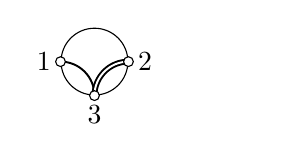
\begin{tikzpicture}
  [ scale = 0.6,
    thin,
    inner/.style={circle,draw=black!100,fill=black!100,inner sep=1.25pt},
    attach/.style={circle,draw=black!100,fill=black!0,thin,inner sep=1.25pt},
    sin/.style={line width=.7pt},
    doub/.style={line width=2.1pt},
    trip/.style={draw=white,line width=.7pt}]
    \node at (0,0){};
%\begin{scope}[yshift=1.8cm]
%  \node (2)  at (0,0) [attach,label=left:3] {};
%  \node (1)  at (0,1) [attach,label=left:1] {};
%  \node (3)  at (3,1) [attach,label=right:2] {};
%  \node (4)  at (1,0) [inner]  {};
%  \node (5)  at (2,0) [inner]  {};
%  \node (6)  at (1,1) [inner]  {};
%  \node (7)  at (2,1) [inner]  {};
%  \node (8)  at (2,2) [inner]  {};
%  \node (9)  at (2.866,2.5)  [inner] {};
%  \node (10) at (1.134,2.5)  [inner] {};
%  \node (11) at (2,-1)       [inner] {};
%  \node (12) at (2.866,-1.5) [inner] {};
%  \node (13) at (1.134,-1.5) [inner] {};
%
%  \draw (2) to (4);
%  \draw (4) to (5);
%  \draw (3) to (7);
%  \draw (1) to (6);
%  \draw (6) to (4);
%  \draw (6) to (7);
%  \draw (7) to (5);
%  \draw (7) to (8);
%  \draw (8) to (9);
%  \draw (8) to (10);
%  \draw (11) to (5);
%  \draw (11) to (12);
%  \draw (11) to (13);
%
  \node (split) at (-3.6,.8) [draw=black,circle,inner sep=3mm,
         label=left:1,label=right:2,label=below:3] {};
% 
%  \node at (-1.6,.5) {=};

  \draw[sin]  (split.west) to[out=0,in=90]   (split.south);
  \draw[doub] (split.east) to[out=180,in=90] (split.south);
  \draw[trip] (split.east) to[out=180,in=90] (split.south);
  
  \node at (split.east) [attach] {};
  \node at (split.west) [attach] {};
  \node at (split.south) [attach]{};
%\end{scope}
\end{tikzpicture}
  \label{fig:mom_switch}
}
\hspace{0.5cm}
\subfloat[][]{
  \tikzsetnextfilename{MP_u_cd_gate}
  \begin{tikzpicture}
  [ scale = 1,
    yscale = .8,
    attach/.style={circle,draw=black!100,fill=white,thick,
    minimum size = 6mm},
    cross/.style={line width=4pt, draw=white},
    drawn/.style={draw=black},
    vert/.style = {circle,fill=black,inner sep=.6pt, minimum size=0},
    nofill/.style = {circle,draw=black,fill=white,inner sep = 1.25pt,minimum size=0},
    decoration={markings,
		mark=between positions 0 and 10 step .1cm
 		with { \node at (0,0) [vert]{}; }}]

  \node (bottom) at ( 1, 0) [attach] {};
  \node (top)    at ( 1, 2.5) [attach] {};
  
  \foreach \x in {0,.1,...,3.5}{
  \foreach \y in {.75, 3.25}{
    \node at (\x,\y) [vert] {};
  }}

  \draw[postaction={decorate}] (0,0) node[left] {$1_{\med,\text{in}}$} 
    -- (bottom.west);
  \draw (0,.75) node [left] {$0_{\med,\text{in}}$} 
    -- (3.5,.75) node [right] {$0_{\med,\text{out}}$};
  \draw (0,3.25) node [left] {$0_{c,\text{in}}$}
    -- (3.5,3.25) node [right] {$0_{c,\text{out}}$};
  \draw[postaction={decorate}] (0,2.5) node [left] {$1_{c,\text{in}}$} 
    -- (top.west) ;
  \draw (top.south) -- (bottom.north) [cross];

  \draw (top.south) -- (bottom.north) [drawn,postaction={decorate}];
  \draw (top.east) -- ( 2, 2.5)  .. controls (2.5,2.5) and (2.5, 0) 
                   .. (3,0) -- (3.5, 0)  [cross];
  \draw (top.east) -- ( 2, 2.5)  .. controls (2.5,2.5) and (2.5, 0) 
                    .. (3,0) -- (3.5, 0) 
                    node [right] {$1_{\med,\text{out}}$} [drawn,postaction={decorate}];
  \draw (bottom.east) -- ( 2, 0) .. controls (2.5,0) and (2.5,2.5)  
                      .. (3,2.5) -- (3.5, 2.5)  [cross];
  \draw[drawn,postaction={decorate}] (bottom.east) -- ( 2, 0) .. controls (2.5,0) and (2.5,2.5)  
                      .. (3,2.5) -- (3.5, 2.5) 
                      node [right] {$1_{c,\text{out}}$} ;

  \draw (top.west) to[out=0,in=90] (top.south) [line width = .7pt];
  \draw (bottom.east) to[out=-180,in=-90] (bottom.north) [line width=.7pt];
  \draw (top.east) to[out=-180,in=90] (top.south) [line width=2.1pt];
  \draw (top.east) to[out=-180,in=90] (top.south) [line width=.7pt,draw=white];
  \draw (bottom.west) to[out=0,in=-90] (bottom.north) [line width=2.1pt];
  \draw (bottom.west) to[out=0,in=-90] (bottom.north) [line width=.7pt,draw=white];  
  
  
  \foreach \x in {0, 3.5}{
  \foreach \y in {0,.75, 2.5, 3.25}{
    \node at (\x,\y) [nofill] {};
  }}
 
 \node at (top.west) [nofill]{};
 \node at (top.east) [nofill]{};
 \node at (top.south) [nofill]{};
 \node at (bottom.west) [nofill]{};
 \node at (bottom.east) [nofill]{};
 \node at (bottom.north) [nofill]{};
  
\end{tikzpicture}
  \label{fig:cd_gate}
}
\caption{\subfig{mom_switch} Momentum switch schematic. \subfig{cd_gate} $\CD$ gate.}

\label{fig:onepsplit}
\end{figure}

\subsubsection{Momentum switch}

Remember from \sec{mom_switch} that momentum switches are three-terminal scattering gadgets that act like railroad switches, where at specific momenta the gadget has perfect transmission from terminal 3 to terminal 1, while at other momenta there is perfect transmission from terminal 3 to terminal 2.  We will represent gadgets with this behavior schematically as in \fig{mom_switch}, where one set of momenta follow the single line while the other specified set follows the double line.

For our purposes, we will assume that the momentum switch splits the two momenta used to encode the different qubits $k_{\text{com}}$ and $k_{\text{med}}$.  Explicitly, we will assume that the $S$-matrix for the given momentum switch at $k_1$ and $k_2$ are given by
\begin{equation}
  S_{\text{switch}}(k_{\text{com}}) = \begin{pmatrix} 0 & 0 & T_{\text{com}}\\
    0 & R_{\text{com}} & 0\\
    T_{\text{com}} & 0 & 0\end{pmatrix}\qquad
  S_{\text{switch}}(k_{\text{med}}) = \begin{pmatrix}R_{\text{med}} & 0 &0\\
    0 & 0 & T_{\text{med}}\\
    0 & T_{\text{med}} & 0\end{pmatrix}.
\label{eq:switch_S}
\end{equation}
In other words, we will assume that the momentum switch has perfect transmission between terminals $1$ and $3$ at momentum $k_{\text{com}}$, and perfect transmission between terminals $2$ and $3$ at momentum $k_{\text{med}}$, possibly with an additional phase.  With this, we have that a particle with momentum $k_{\text{com}}$ follows the single line, while a particle with momentum $k_{\text{med}}$ follows the double line.


\subsubsection{Constructing the graph}

We will now construct this graph, where we will assume that we know the encoded initial states.  Note that this construction doe depend on the momenta of the encoded qubits in more than just the form of the momentum switch; the fact that the timing of the wave-packets is important forces us to change the length of the connecting paths depending on the initial momentum so that they arrive on the infinite path at the same time, while the requirement that the particles only interact along the path forces us to change the lengths depending on the size of the wave-packets.

The $\CD$ gate is implemented using the graph shown in \fig{explicit_cd}. In this section we specify the logical input states, the logical output states, the distances $X$, $Z$, and $W$ appearing in the figure, and the total evolution time as functions of the momentum $k_{\text{com}}$ and $k_{\text{med}}$. With these choices, we show that a $\CD$ gate is applied to the logical states at the end of the time evolution under the quantum walk Hamiltonian (up to error terms that are $\tilde{\O}(L^{-{1}/{2}})$). The results of this section pertain to the two-particle Hamiltonian $H^{(2)}_{G'}$ for the graph $G'$ shown in \fig{explicit_cd}.
\todo{get correct error term}

We first need to construct the assumed encoded initial states.  
\begin{align}
|0_{\text{in}}\rangle^{\text{com}}&=  \gamma \sum_{x = \mu -L} ^{\mu + L}  e^{i k_{\text{com}} x} e^{- \frac{(x-\mu)^2}{2\sigma^2}} \ket{x,1} & |1_\text{in}\rangle^c&= \gamma \sum_{x = \mu -L} ^{\mu + L}  e^{i k_{\text{com}} x} e^{- \frac{(x-\mu)^2}{2\sigma^2}} \ket{x,2} 
\end{align}
for the computational qubit and
\begin{equation*}
|0_{\text{in}}\rangle^\med=\gamma \sum_{x = \nu -L} ^{\nu + L}  e^{i k_{\text{med}} x} e^{- \frac{(x-\nu)^2}{2\sigma^2}} \ket{x,4} \qquad |1_\text{in}\rangle^\med=\gamma \sum_{x = \nu -L} ^{\nu + L}  e^{i k_{\text{med}} x} e^{- \frac{(x-\nu)^2}{2\sigma^2}} \ket{x,3} 
\end{equation*}
 for the mediator qubit. We can then define symmetrized (or antisymmetrized) logical input states for $a,b\in\{0,1\}$ as
\begin{align*}
|a b_{\text{in}}\rangle^{\text{com},\med}_\pm &=\frac{1}{\sqrt{2}} \left(|a_{\text{in}}\rangle^{\text{com}} |b_{\text{in}}\rangle^\med \pm |b_{\text{in}}\rangle^\med|a_{\text{in}}\rangle^{\text{com}}\right).
\end{align*}

\begin{figure}
  \centering
  \tikzsetnextfilename{MP_u_explicit_cd}
  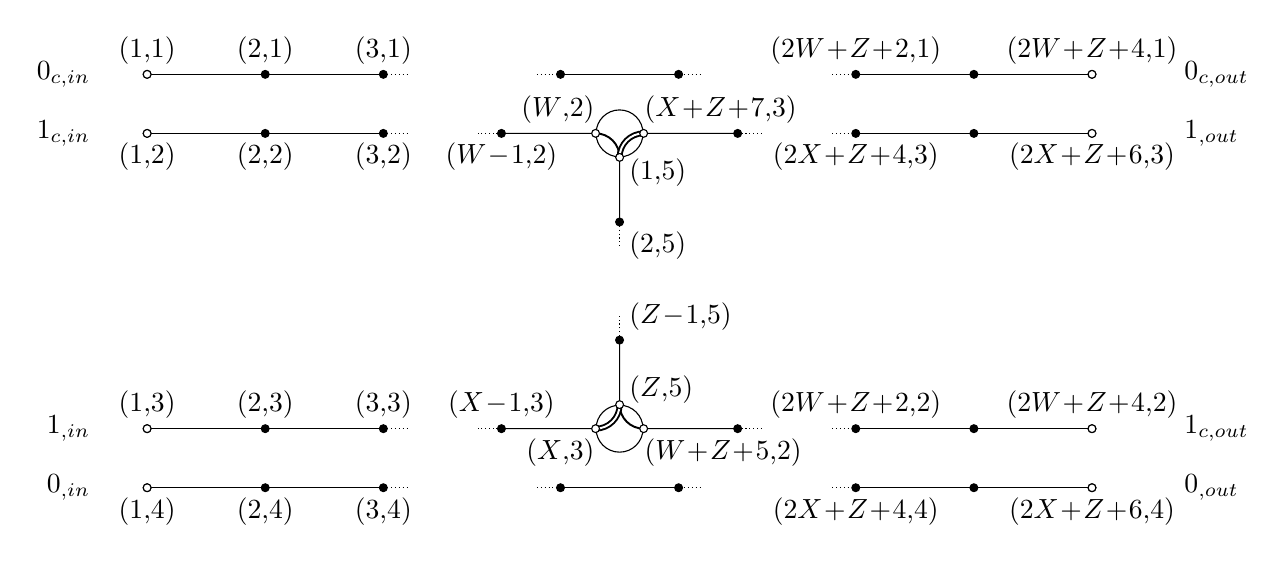
\begin{tikzpicture} [scale=1.5,
	vert/.style={circle, draw=black, fill=black,inner sep=1pt, minimum width=0pt},
	dots/.style={circle, fill=black,inner sep=1pt, minimum width=0pt},
	switch/.style={circle,draw=black,inner sep=6pt,minimum width=0pt},
	attach/.style={circle,fill=white, draw=black,inner sep=1pt, minimum width=0pt}]

  \foreach \y in {0,0.5,3,3.5}{
  \begin{scope}[yshift=\y cm]
  \foreach \x in {0,1,2,6,7,8}{
	\begin{scope}[xshift = \x cm]
	  \node at (0,0) [vert]{};
	\end{scope}}
	\draw (0,0) -- (2,0);
	\draw (6,0) -- (8,0);
	\draw[densely dotted] (2,0)--(2.2,0);
	\draw[densely dotted] (5.8,0)--(6,0);
	\node at (0,0) [attach] {};
	\node at (8,0) [attach] {};
 \end{scope}}
 
  
  \node (switch2) at (4,0.5)[switch]{};
  \node (switch1) at (4,3)[switch]{};
  
  \node at (3,0.5) [vert]{};
  \node at (3,3) [vert]{};
  \node at (5,0.5) [vert]{};
  \node at (5,3) [vert]{};
  
  \draw (switch2.west) -- (3,0.5);
  \draw[densely dotted] (3,0.5) -- (2.8,0.5);
  \draw (switch2.east) -- (5,0.5);
  \draw[densely dotted] (5,0.5) -- (5.2,0.5);
  
  \draw (switch1.west) -- (3,3);
  \draw[densely dotted] (3,3) -- (2.8,3);
  \draw (switch1.east) -- (5,3);
  \draw[densely dotted] (5,3) -- (5.2,3);
  
  \node at (3.5,0) [vert]{};
  \node at (4.5,0) [vert]{};
  \node at (3.5,3.5) [vert]{};
  \node at (4.5,3.5) [vert]{};
  
  \draw (3.5,0) -- (4.5,0);
  \draw (3.5,3.5) -- (4.5,3.5);
  \draw[densely dotted] (3.3,0) -- (4.7,0);
  \draw[densely dotted] (3.3,3.5) -- (4.7,3.5);
  

  \node at (4,1.25) [vert] {};
  \node at (4,2.25) [vert] {};
  
  \draw (switch2.north) -- (4,1.25);
  \draw[densely dotted] (4,1.25) -- (4,1.45);
  
  \draw (switch1.south) -- (4,2.25);
  \draw[densely dotted] (4,2.25)-- (4,2.05);
  
  \draw[line width=.7pt] (switch1.west) to[out=0,in=90] (switch1.south);
  \draw[line width=2.1pt] (switch1.east) to[out=180,in=90] (switch1.south);
  \draw[line width=.7pt,white] (switch1.east) to[out=180,in=90] (switch1.south);

  \draw[line width=.7pt] (switch2.east) to[out=180,in=-90] (switch2.north);
  \draw[line width=2.1pt] (switch2.west) to[out=0,in=-90] (switch2.north);
  \draw[line width=.7pt,white] (switch2.west) to[out=0,in=-90] (switch2.north);
  
  \node at (switch2.north) [attach] {};
  \node at (switch1.south) [attach] {};
  \node at (switch2.east) [attach] {};
  \node at (switch1.east) [attach] {};
  \node at (switch2.west) [attach] {};
  \node at (switch1.west) [attach] {};
  
  \node at (0,0) [below] {(1,4)};
  \node at (1,0) [below] {(2,4)};
  \node at (2,0) [below] {(3,4)};
  \node at (3.5,0) [below] {};
  \node at (4.5,0) [below] {};
  \node at (6,0) [below] {($2X\!+\! Z\! + \! 4$,4)};
  \node at (8,0) [below] {($2X\! +\! Z\! +\! 6$,4)};
  
  \node at (0,3.5) [above] {(1,1)};
  \node at (1,3.5) [above] {(2,1)};
  \node at (2,3.5) [above] {(3,1)};
  \node at (3.5,3.5) [above] {};
  \node at (4.5,3.5) [above] {};
  \node at (6,3.5) [above] {($2W\! + \! Z\! + \! 2$,1)};
  \node at (8,3.5) [above] {($2W\! + \! Z\! + \! 4$,1)};
  
  \node at (0,3) [below] {(1,2)};
  \node at (1,3) [below] {(2,2)};
  \node at (2,3) [below] {(3,2)};
  \node at (3,3) [below] {($W\!-\! 1$,2)};
  \node[anchor=south east] at (3.87,3) {($W$,2)};
  
  \node at (0,.5) [above] {(1,3)};
  \node at (1,.5) [above] {(2,3)};
  \node at (2,.5) [above] {(3,3)};
  \node at (3,.5) [above] {($X\! -\! 1$,3)};
  \node at (3.87,.5) [below left] {($X$,3)};
  
  \node at (8,.5) [above] {($2W\! + \! Z\! + \! 4$,2)};
  \node at (6,.5) [above] {($2W\! + \! Z\! + \! 2$,2)};
  \node at (4.13,.5) [below right] {($W\! + \! Z\! + \! 5$,2)};  
  
  \node at (8,3) [below] {($2X\! + \! Z\! + \! 6$,3)};
  \node at (6,3) [below] {($2X\! + \! Z\! + \! 4$,3)};
  \node at (4.13,3) [above right] {($X\! + \! Z\! + \! 7$,3)};
  
  \node at (4,2.87) [below right] {(1,5)};
  \node at (4,2.25) [below right] {(2,5)};
  
  \node at (4,.63) [above right] {($Z$,5)};
  \node at (4,1.25) [above right] {($Z\! -\! 1$,5)};
  
  \node at (-.4,0) [left] {$0_{\med,\text{in}}$};
  \node at (-.4,.5) [left] {$1_{\med,\text{in}}$};
  \node at (-.4,3) [left] {$1_{c,\text{in}}$};
  \node at (-.4,3.5) [left] {$0_{c,\text{in}}$};
  
  \node at (8.7,0) [right] {$0_{\med,\text{out}}$};
  \node at (8.7,.5) [right] {$1_{c,\text{out}}$};
  \node at (8.7,3) [right] {$1_{\med,\text{out}}$};
  \node at (8.7,3.5) [right] {$0_{c,\text{out}}$};
\end{tikzpicture} 
  \caption{Graph $G'$ used to implement the $\CD$ gate. The integers $Z$, $X$, and $W$ are specified in equations \eq{Z_eq}, \eq{X_eq}, and \eq{W_eq}, respectively.}
\label{fig:explicit_cd}
\end{figure}

We choose the distances $Z$, $X$, and $W$ from \fig{Graph-used-to-1}
to be \begin{align}
Z & = 4L \label{eq:Z_eq} \\
X & = d_{2}+L+M\left(-\frac{\pi}{2}\right) \label{eq:X_eq}\\
W & = d_{1}+L+M\left(-\frac{\pi}{4}\right) \label{eq:W_eq}
\end{align}
where
\begin{align*}
d_{1} & = M\left(-\frac{\pi}{4}\right) \\
d_{2} & = \left\lceil \frac{5L+2d_{1}}{\sqrt{2}}-\frac{5}{2}L\right\rceil. \end{align*}
With these choices, a wave packet moving with speed $\sqrt{2}$ travels
a distance $Z+2d_{1}+L=5L+2d_{1}$ in approximately the same time that
a wave packet moving with speed $2$ takes to travel a distance $Z+2d_{2}+L=5L+2d_{2}$,
since
\begin{align}
t_{\mathrm{II}}=\frac{5L+2d_{1}}{\sqrt{2}}\approx\frac{5L+2d_{2}}{2}.
\end{align}

We claim that the logical input states evolve into logical output states (defined below) with a phase of $e^{i\theta}$ applied in the case where both particles are in the logical state $1$.  Specifically, let us define the output states as, 
\begin{align*}
|0_\text{out}\rangle^c &=\frac{e^{-it_{\mathrm{II}}\sqrt{2}}}{\sqrt{L}}\sum_{x=Q_{1}+1}^{Q_{1}+L}e^{-i\frac{\pi}{4}x}|x,1\rangle &
|1_\text{out}\rangle^c &=\frac{e^{-it_{\mathrm{II}}\sqrt{2}}}{\sqrt{L}}\sum_{x=Q_{1}+1}^{Q_{1}+L}e^{-i\frac{\pi}{4}x}|x,2\rangle \\
|0_\text{out}\rangle^\med &=\frac{1}{\sqrt{L}}\sum_{y=Q_{2}+1}^{Q_{2}+L}e^{-i\frac{\pi}{2}y}|y,4\rangle &|1_\text{out}\rangle^\med &=\frac{1}{\sqrt{L}}\sum_{y=Q_{2}+1}^{Q_{2}+L}e^{-i\frac{\pi}{2}y}|y,3\rangle
\end{align*}
where  $Q_{1}=2W+Z+4-M\left(-{\pi}/{4}\right)-L$ and $Q_{2}=2X+Z+6-M\left(-{\pi}/{2}\right)-L$,and $|a b_\text{out}\rangle^{c,\med}=\text{Sym}\left(|a_{\text{out}}\rangle^c|b_{\text{out}}\rangle^\med\right)$. 

Note that the input states are wave packets located a distance $M(k)$ from the ends of the input paths on the left-hand side of the graph in \fig{Graph-used-to-1}. Similarly, the output logical states are wave packets located a distance $M(k)$ from the ends of the output paths on the right-hand side.

We then have the following lemma:
\begin{lemma}
For the graph given in \fig{explicit_cd}, we have the following bounds for the time-evolved states:
\begin{align}
\left\Vert e^{-iH_{G'}^{(2)}t_{\mathrm{II}}}|00_{\text{in}}\rangle^{c,\med}-|00_{\text{out}}\rangle^{c,\med}\right\Vert  & = \O(L^{-{1}/{4}})\label{eq:bound00}\\
\left\Vert e^{-iH_{G'}^{(2)}t_{\mathrm{II}}}|01_{\text{in}}\rangle^{c,\med}-|01_{\text{out}}\rangle^{c,\med}\right\Vert  & = \O(L^{-{1}/{4}})\label{eq:bound01}\\
\left\Vert e^{-iH_{G'}^{(2)}t_{\mathrm{II}}}|10_{\text{in}}\rangle^{c,\med}-|10_{\text{out}}\rangle^{c,\med}\right\Vert  & = \O(L^{-{1}/{4}})\label{eq:bound10}\\
\left\Vert e^{-iH_{G'}^{(2)}t_{\mathrm{II}}}|11_{\text{in}}\rangle^{c,\med} - e^{i\theta}|11_{\text{out}}\rangle^{c,\med}\right\Vert  & = \O(L^{-{1}/{4}}).\label{eq:bound11}
\end{align}
\end{lemma}


\begin{proof}
The first three bounds \eq{bound00}, \eq{bound01}, and \eq{bound10} are relatively easy to show, since in each case the two particles are supported on disconnected subgraphs and therefore do not interact. In each of these three cases we can simply analyze the propagation of the one-particle starting states through the graph. The symmetrized (or antisymmetrized) starting state then evolves into the symmetrized (or antisymmetrized) tensor product of the two output states.

For example, with input state $|00_{\text{in}}\rangle^{c,\med}$, the evolution of the particle with momentum $-{\pi}/{4}$ occurs only on the top path and the evolution of the particle with momentum $-{\pi}/{2}$ occurs only on the bottom path. Starting from the initial state $|0_\text{in}\rangle^c$ and evolving for time $t_{\mathrm{II}}$ with the single-particle Hamiltonian for the top path, we obtain the final state
\begin{align}
|0_\text{out}\rangle^c+\O(L^{-{1}/{4}})
\end{align}
using the method of \sec{truncating}. Similarly, starting from the initial state $|0_\text{in}\rangle^\med$ and evolving for time $t_{\mathrm{II}}$ with the single-particle Hamiltonian
for the bottom path of the graph we obtain the final state
\begin{align}
|0_\text{out}\rangle^{\med}+\O(L^{-{1}/{4}}).
\end{align}
Putting these bounds together we get the bound \eq{bound00}.

In the case where the input state is $|10_{\text{in}}\rangle^{c,\med}$ (or $|01_{\text{in}}\rangle^{c,\med}$) the single-particle evolution for the particle with momentum $-{\pi}/{4}$ (or $-{\pi}/{2}$) is slightly more complicated, as in this case the particle moves through the momentum switches and the vertical path. The S-matrix of the momentum switch at the relevant momenta is given by equation \eq{switch_S}. At momentum $-{\pi}/{4}$, the momentum switch has the same S-matrix as a path with $4$ vertices (including the input and output vertices). At momentum $-{\pi}/{2}$, it has the same S-matrix as a path with $5$ vertices (including input and output vertices). Note that our labeling of vertices on the output paths (in \fig{Graph-used-to-1}) takes this into account. The first vertices on the output paths connected to the momentum switches are labeled $(X+Z+7,3)$ and $(W+Z+5,2)$, respectively, reflecting the fact that a particle with momentum $-{\pi}/{4}$ has traveled $W$ vertices on the input path, $Z$ vertices through the middle segment, and has effectively traveled an additional $4$ vertices inside the two switches. Similarly, a particle with momentum $-{\pi}/{2}$ effectively sees an additional $6$ vertices from the two momentum switches.

To get the bound \eq{bound10} we have to analyze the single-particle evolution
for the computational particle initialized in the state $|1_\text{in}\rangle^c$. 
We claim that, after time $t_{\mathrm{II}}$, the time-evolved state is
\begin{align}
|1_\text{out}\rangle^c+\O(L^{-{1}/{4}}).
\end{align}
It is easy to see why this should be the case in light of our discussion above: when scattering at momentum $-{\pi}/{4}$, the graph in \fig{Graph-used-to-1} is equivalent to one where each momentum switch is replaced by a path with $2$ internal vertices connecting the relevant input/output vertices.

To make this precise, we use the method described in \sec{more_complicated_graphs} for analyzing scattering through sequences of overlapping graphs using the truncation lemma. Here we should choose subgraphs $G_{1}$ and $G_{2}$ of the graph $G'$ in \fig{Graph-used-to-1} that overlap on the vertical path but where each subgraph contains only one of the momentum switches. A convenient choice is to take $G_{1}$ to be the subgraph containing the top switch and the paths connected to it (the vertices $(1,2),\ldots,(W,2)$, $(1,5),\ldots,(Z,5)$ and $(X+Z+7,3),\ldots,(2X+Z+6,3)$). Similarly, choose $G_{2}$ to be the bottom switch along with the three paths connected to it. The graphs $G_{1}$ and $G_{2}$ both contain the vertices $(1,5),\ldots,(Z,5)$ along the vertical path. Break up the total evolution time into two intervals $[0,t_{\alpha}]$ and $[t_{\alpha},t_{\mathrm{II}}]$. Choose $t_{\alpha}$ so that the wave packet, evolved for this time with $H_{G_1}^{(1)}$, travels through the top switch and ends up a distance $\Theta(L)$ from each switch, partway along the vertical path (up to terms bounded as $\O(L^{-{1}/{4}})$, as in \sec{truncating}). With this choice, the single-particle evolution with the Hamiltonian for the full graph is approximated by the evolution with $H_{G_1}^{(1)}$ on this time interval (see \sec{more_complicated_graphs}). At time $t_\alpha$, the particle is outgoing with respect to scattering from the graph $G_1$, but incoming with respect to $G_2$. On the interval $[t_{\alpha},t_{\mathrm{II}}]$ the time evolution is approximated by evolving the state with $H_{G_2}^{(1)}$. During this time interval the particle travels through the bottom switch onto the final path, and at $t_{\mathrm{II}}$ is a distance $M(-{\pi}/{4})$ from the endpoint of the output path. Both switches have the same S-matrix (at momentum $-{\pi}/{4}$) as a path of length $4$, so this analysis gives the output state $|10_\text{out}\rangle^{c,\med}$ up to terms bounded as $\O(L^{-{1}/{4}})$, establishing \eq{bound10}. For the bound \eq{bound01}, we apply a similar analysis to the trajectory of the mediator particle.

The case where the input state is $|11_{\text{in}}\rangle^{c,\med}$ is more involved but proceeds similarly. In this case, to analyze the time evolution we divide the time interval $[0,t_{\mathrm{II}}]$ into three segments $[0,t_{A}]$, $[t_{A},t_{B}]$, and $[t_{B},t_{\mathrm{II}}]$. For each of these three time intervals we choose a subgraph $G_{A}$, $G_{B}$, $G_C$ of the graph $G'$ in \fig{Graph-used-to-1} and we approximate the time evolution by evolving with the Hamiltonian on the associated subgraph. We then use the truncation lemma to show that, on each time interval, the evolution generated by the Hamiltonian for the appropriate subgraph approximates the evolution generated by the full Hamiltonian, with error $\O(L^{-{1}/{4}})$. Up to these error terms, at times $t=0$, $t=t_A$, $t=t_B$, and $t=t_{\mathrm{II}}$ the time-evolved state 
\begin{align}
e^{-iH_{G'}^{(2)}t}|11_{\text{in}}\rangle^{c,\med}
\end{align}
has both particles in square wave packet states, each with support only on $L$ vertices of the graph, as depicted in \fig{11_scattering_cartoon}.

We take $G_A$ to be the subgraph obtained from $G'$ by removing the vertices labeled $(\lceil 1.85L\rceil,5)\allowbreak, \ldots,\allowbreak (\lceil 1.90 L\rceil,5)$ in the vertical path. By removing this interval of consecutive vertices, we disconnect the graph into two components where the initial state $|11_{\text{in}}\rangle^{c,\med}$ has one particle in each component. This could be achieved by removing a single vertex, but instead we remove an interval of approximately $0.05L$ vertices to separate the components of $G_A$ by more than the interaction range $C$ (for sufficiently large $L$), simplifying our use of the truncation lemma.

 We choose $t_{A}={3L}/{2}$. Consider the time evolution of the initial state $|11_\text{in}\rangle^{c,\med}$ with the two-particle Hamiltonian $H_{G_A}^{(2)}$ for time $t_A$. The states $|1_ {\text{in}}\rangle^c$ and $|1_\text{in}\rangle^{\med}$ are supported on disconnected components of the graph $G_A$, so we can analyze the time evolution of the state $|11_\text{in}\rangle^{c,\med}$ under $H_{G_A}^{(2)}$ by analyzing two single-particle problems, using the results of \sec{truncating} for each particle. During the interval $[0,t_A]$,  each particle passes through one switch, ending up a distance $\Theta(L)$ from the switch that it passed through and $\Theta(L)$ from the vertices that have been removed, as shown in \fig{11_scattering_cartoon}(b) (with error at most $\O(L^{-{1}/{4}})$). Up to these error terms, the support of each particle remains at least $N_0=\Theta(L)$ vertices from the endpoints of the graph, so we can apply the truncation lemma using $H=H_{G'}^{(2)}$, $W=\tilde{H}=H_{G_A}^{(2)}$, $T=t_{\mathrm{A}}$, and $\delta=\O(L^{-{1}/{4}})$. Here $P$ is the projector onto states where both particles are located at vertices of $G_A$. We have $P H_{G'}^{(2)}P=H_{G_A}^{(2)}$ since the number of vertices in the removed segment is greater than the interaction range $C$. Applying the truncation lemma gives
\begin{align}
\left\Vert e^{-iH_{G_A}^{(2)}t_A}|11_\text{in}\rangle^{c,\med}-e^{-iH_{G'}^{(2)}t_A}|11_\text{in}\rangle^{c,\med}\right\Vert=\O(L^{-{1}/{4}}).
\end{align}

We approximate the evolution on the interval $[t_A,t_B]$ using the two-particle  Hamiltonian $H_{G_B}^{(2)}$, where $G_B$  is the vertical path $(1,5),\ldots,(Z,5)$. Using the result of \sec{truncating}, we know that (up to terms bounded as $\O(L^{-{1}/{4}})$) the wave packets move with their respective speeds and acquire a phase of $e^{i\theta}$ as they pass each other. We choose $t_B={5L}/{2}$ so that during the evolution the wave packets have no support on vertices within a distance $\Theta(L)$ from the endpoints of the vertical segment where the graph has been truncated (again up to terms bounded as $\O(L^{-{1}/{4}})$). Using $H_{G_B}^{(2)}$ (rather than $H_{G'}^{(2)}$) to evolve the state on this interval, we incur errors bounded as $\O(L^{-{1}/{4}})$ (using the truncation lemma with $N_0=\Theta(L)$, $W=\tilde{H}=H_{G_B}^{(2)}$, $H=H_{G'}^{(2)}$, and $\delta=\O(L^{-{1}/{4}})$).

We choose $G_C=G_A$; in the final interval $[t_{B},t_{\mathrm{II}}]$ we evolve using the Hamiltonian  $H_{G_A}^{(2)}$ again, and we use the truncation lemma as we did for the first interval. The initial state is approximated by two wave packets supported on disconnected sections of $G_A$ and the evolution of this initial state reduces to two single-particle scattering problems. During the interval $[t_B,t_{\mathrm{II}}]$, each particle passes through a second switch, and at time $t_{\mathrm{II}}$ is a distance $M(k)$ from the end of the appropriate output path. 

Our analysis shows that for the input state $|11_\text{in}\rangle^{c,\med}$ the only effect of the interaction is to alter the global phase of the final state by a factor of $e^{i\theta}$ relative to the case where no interaction is present, up to error terms bounded as $\O(L^{-{1}/{4}})$. This establishes equation \eq{bound11}. In \fig{11_scattering_cartoon} we illustrate the movement of the two wave packets through the graph when the initial state is $|11_\text{in}\rangle^{c,\med}$.

\end{proof}

\todo{split 11\_scattering\_cartoon into several subfigures}

\begin{figure}
  \centering
  \tikzsetnextfilename{MP_u_11_scattering_cartoon}
  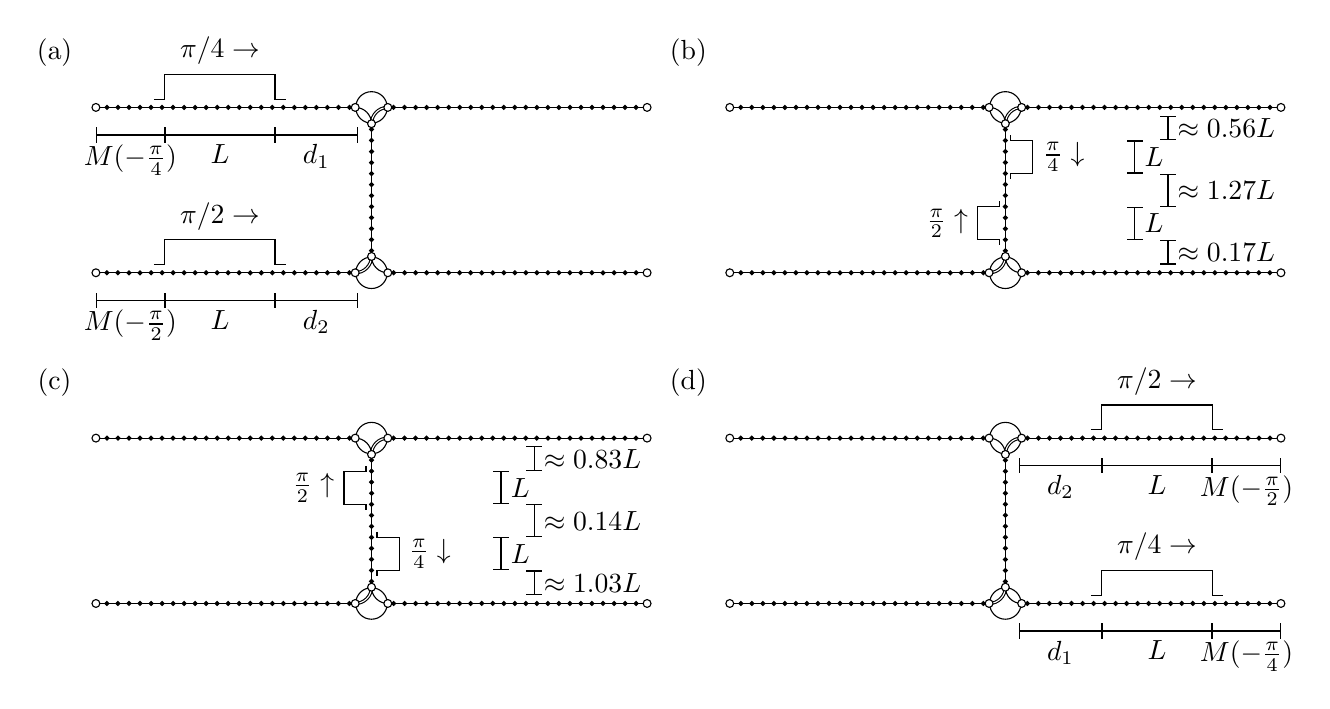
\begin{tikzpicture}[   scale=0.7,   
	dots/.style={circle,draw=black,fill=black,inner sep=0pt,minimum size=.5 mm}, 
	splitter/.style={circle,draw=black,fill=white,inner sep=0pt,minimum size=4mm},   
	attach/.style={circle,draw=black,fill=white,inner sep=0pt,minimum size=1mm}]
	
\begin{scope}[yshift= 6 cm]
  \node at (-.75,4) {(a)};

  \draw (0,0) to (10,0);   
  \draw (0,3) to (10,3);
  \foreach \x in {0,.2,.4,...,10}{
  \node at (\x, 0) [dots] {};
  \node at (\x, 3) [dots] {};
  }
  \foreach \y in {0,.2,.4,...,3}
  \node at (5,\y) [dots] {};
  
  \node (splitter42) at (5,0) [splitter] {};   
  \node (splitter41) at (5,3) [splitter] {};   
  \draw (splitter41.south) to (splitter42.north);      
  \draw (splitter41.west) to[out=0,in=90] (splitter41.south);   
  \draw[line width=1.2pt] (splitter41.south) to[out=90,in=180]           
  (splitter41.east);   
  \draw[line width=.4pt,white] (splitter41.south) to[out=90,in=180] (splitter41.east);
  \draw[line width=1.2pt] (splitter42.west) to[out=0,in=-90]           (splitter42.north);   
  \draw[line width=.4pt,white] (splitter42.west) to[out=0,in=-90]           (splitter42.north);   
  \draw (splitter42.north) to[out=-90,in=180] (splitter42.east);
  \node at (splitter41.east) [attach]{};
  \node at (splitter41.west) [attach]{};
  \node at (splitter41.south) [attach]{};
  \node at (splitter42.east) [attach]{};
  \node at (splitter42.west) [attach]{};
  \node at (splitter42.north) [attach]{};
  
  \node at (0,0) [attach]{};
  \node at (0,3) [attach]{};
  \node at (10,0) [attach]{};
  \node at (10,3) [attach]{};  

  \draw (1.05,3.15) to (1.25,3.15) to (1.25,3.6) to node[above]          
    {${\pi}/{4}\rightarrow$} (3.25,3.6) to (3.25,3.15) to (3.45,3.15);
  \draw (1.05,0.15) to (1.25,0.15) to (1.25,0.6) to node[above]          
    {${\pi}/{2}\rightarrow$} (3.25,0.6) to (3.25,0.15) to (3.45,0.15);
  \draw[|-|] (0,2.5) to node[below] {$M(-\frac{\pi}{4})$} (1.25,2.5);   
  \draw[|-|] (1.25,2.5) to node[below]{$L$}   (3.25,2.5);   
  \draw[|-|] (3.25,2.5) to node[below]{$d_1$} (4.75,2.5);
  \draw[|-|] (0,-.5) to node[below] {$M(-\frac{\pi}{2})$} (1.25,-.5);   
  \draw[|-|] (1.25,-.5) to node[below]{$L$}   (3.25,-.5);   
  \draw[|-|] (3.25,-.5) to node[below]{$d_2$} (4.75,-.5);
\end{scope}
  
%----------------------------------------------------------------------------------------%

\begin{scope}[xshift= 11.5cm, yshift=6cm]
  \node at (-.75,4) {(b)};

  \draw (0,0) to (10,0);   
  \draw (0,3) to (10,3);
  \foreach \x in {0,.2,.4,...,10}{
  \node at (\x, 0) [dots] {};
  \node at (\x, 3) [dots] {};
  }
  \foreach \y in {0,.2,.4,...,3}
  \node at (5,\y) [dots] {};
  
  \node (splitter42) at (5,0) [splitter] {};   
  \node (splitter41) at (5,3) [splitter] {};   
  \draw (splitter41.south) to (splitter42.north);      
  \draw (splitter41.west) to[out=0,in=90] (splitter41.south);   
  \draw[line width=1.2pt] (splitter41.south) to[out=90,in=180]           
  (splitter41.east);   
  \draw[line width=.4pt,white] (splitter41.south) to[out=90,in=180] (splitter41.east);
  \draw[line width=1.2pt] (splitter42.west) to[out=0,in=-90]           (splitter42.north);   
  \draw[line width=.4pt,white] (splitter42.west) to[out=0,in=-90]           (splitter42.north);   
  \draw (splitter42.north) to[out=-90,in=180] (splitter42.east);
  \node at (splitter41.east) [attach]{};
  \node at (splitter41.west) [attach]{};
  \node at (splitter41.south) [attach]{};
  \node at (splitter42.east) [attach]{};
  \node at (splitter42.west) [attach]{};
  \node at (splitter42.north) [attach]{};
  
  \node at (0,0) [attach]{};
  \node at (0,3) [attach]{};
  \node at (10,0) [attach]{};
  \node at (10,3) [attach]{};
  \begin{scope}[yshift = -10 cm]
    \draw (5.1,11.7) to (5.1,11.8) to (5.5,11.8) to node[right]          
      {$\frac{\pi}{4}\downarrow$} (5.5,12.4) to (5.1,12.4) to (5.1,12.5);
    \draw (4.9,11.3) to (4.9,11.2) to (4.5,11.2) to node[left]            
      {$\frac{\pi}{2}\uparrow$} (4.5,10.6) to (4.9,10.6) to (4.9,10.5);
    \draw[|-|] (7.95,12.85) to node[right] {$\approx 0.56L$} (7.95,12.4);   
    \draw[|-|] (7.35,12.4)  to node[right] {$L$}   (7.35,11.8);   
    \draw[|-|] (7.95,11.8)  to node[right] {$\approx 1.27L$} (7.95,11.2);   
    \draw[|-|] (7.35,11.2)  to node[right] {$L$}   (7.35,10.6);   
    \draw[|-|] (7.95,10.6)  to node[right] {$\approx 0.17L$} (7.95,10.15);
   \end{scope}  
\end{scope} 
  
%----------------------------------------------------------------------------------------%

  \node at (-.75,4) {(c)};

  \draw (0,0) to (10,0);   
  \draw (0,3) to (10,3);
  \foreach \x in {0,.2,.4,...,10}{
  \node at (\x, 0) [dots] {};
  \node at (\x, 3) [dots] {};
  }
  \foreach \y in {0,.2,.4,...,3}
  \node at (5,\y) [dots] {};
  
  \node (splitter42) at (5,0) [splitter] {};   
  \node (splitter41) at (5,3) [splitter] {};   
  \draw (splitter41.south) to (splitter42.north);      
  \draw (splitter41.west) to[out=0,in=90] (splitter41.south);   
  \draw[line width=1.2pt] (splitter41.south) to[out=90,in=180]           
  (splitter41.east);   
  \draw[line width=.4pt,white] (splitter41.south) to[out=90,in=180] (splitter41.east);
  \draw[line width=1.2pt] (splitter42.west) to[out=0,in=-90]           (splitter42.north);   
  \draw[line width=.4pt,white] (splitter42.west) to[out=0,in=-90]           (splitter42.north);   
  \draw (splitter42.north) to[out=-90,in=180] (splitter42.east);
  \node at (splitter41.east) [attach]{};
  \node at (splitter41.west) [attach]{};
  \node at (splitter41.south) [attach]{};
  \node at (splitter42.east) [attach]{};
  \node at (splitter42.west) [attach]{};
  \node at (splitter42.north) [attach]{};
 
  \node at (0,0) [attach]{};
  \node at (0,3) [attach]{};
  \node at (10,0) [attach]{};
  \node at (10,3) [attach]{};
  \begin{scope}[yshift = - 5cm]
  \draw (5.1,6.3) to (5.1,6.20) to (5.5,6.20) to node[right]            {$\frac{\pi}{4}\downarrow$} (5.5,5.6) to (5.1,5.6) to (5.1,5.5);
  \draw (4.9,6.7) to (4.9,6.8) to (4.5,6.8) to node[left]            {$\frac{\pi}{2}\uparrow$} (4.5,7.4) to (4.9,7.4) to (4.9,7.5);
  \draw[|-|] (7.95,7.85) to node[right] {$\approx 0.83L$} (7.95,7.4);   
  \draw[|-|] (7.35,7.4)  to node[right] {$L$}   (7.35,6.8);   
  \draw[|-|] (7.95,6.8)  to node[right] {$\approx 0.14L$} (7.95,6.2);   
  \draw[|-|] (7.35,6.2)  to node[right] {$L$}   (7.35,5.6);   
  \draw[|-|] (7.95,5.6)  to node[right] {$\approx 1.03L$} (7.95,5.15);
  \end{scope}
  
%----------------------------------------------------------------------------------------%
\begin{scope}[xshift=11.5cm]
  \node at (-.75,4) {(d)};

  \draw (0,0) to (10,0);   
  \draw (0,3) to (10,3);
  \foreach \x in {0,.2,.4,...,10}{
  \node at (\x, 0) [dots] {};
  \node at (\x, 3) [dots] {};
  }
  \foreach \y in {0,.2,.4,...,3}
  \node at (5,\y) [dots] {};
  
  \node (splitter42) at (5,0) [splitter] {};   
  \node (splitter41) at (5,3) [splitter] {};   
  \draw (splitter41.south) to (splitter42.north);      
  \draw (splitter41.west) to[out=0,in=90] (splitter41.south);   
  \draw[line width=1.2pt] (splitter41.south) to[out=90,in=180]           
  (splitter41.east);   
  \draw[line width=.4pt,white] (splitter41.south) to[out=90,in=180] (splitter41.east);
  \draw[line width=1.2pt] (splitter42.west) to[out=0,in=-90]           (splitter42.north);   
  \draw[line width=.4pt,white] (splitter42.west) to[out=0,in=-90]           (splitter42.north);   
  \draw (splitter42.north) to[out=-90,in=180] (splitter42.east);
  \node at (splitter41.east) [attach]{};
  \node at (splitter41.west) [attach]{};
  \node at (splitter41.south) [attach]{};
  \node at (splitter42.east) [attach]{};
  \node at (splitter42.west) [attach]{};
  \node at (splitter42.north) [attach]{};
 
  \node at (0,0) [attach]{};
  \node at (0,3) [attach]{};
  \node at (10,0) [attach]{};
  \node at (10,3) [attach]{};
  \draw (6.55,3.15) to (6.75,3.15) to (6.75,3.6) to node[above]            {${\pi}/{2}\rightarrow$} (8.75,3.6) to (8.75,3.15) to (8.95,3.15);
  \draw (6.55,.15) to (6.75,.15) to (6.75,.6) to node[above]            {${\pi}/{4}\rightarrow$} (8.75,.6)to (8.75,.15) to (8.95,.15);
  \begin{scope}[yshift=-.25cm]
  \draw[|-|] (5.25,2.75) to node[below] {$d_2$} (6.75,2.75);   
  \draw[|-|] (6.75,2.75) to node[below]{$L$}   (8.75,2.75);   
  \draw[|-|] (8.75,2.75) to node[below]{$M(-\frac{\pi}{2})$} (10,2.75);
  \draw[|-|] (5.25,-.25) to node[below] {$d_1$} (6.75,-.25);   
  \draw[|-|] (6.75,-.25) to node[below]{$L$}   (8.75,-.25);   
  \draw[|-|] (8.75,-.25) to node[below]{$M(-\frac{\pi}{4})$} (10,-.25);
  \end{scope}
\end{scope}
\end{tikzpicture} 
  \caption{This picture illustrates the scattering process for two wave packets that are incident on the input paths as shown in figure (a) at time $t=0$. Figure (b) shows the location of the two wave packets after a time $t_{A}={3L}/{2}$ and figure (c) shows the wave packets after a time $t_{B}=t_{A}+L$. After the particles pass one another they acquire an overall phase of $e^{i\theta}$. Figure (d) shows the final configuration of the wave packets after a total evolution time $t_{\mathrm{II}}={(Z+2d_{1}+L)}/{\sqrt{2}}$.}
  \label{fig:11_scattering_cartoon}
\end{figure}






\section{Universal Computation}
\subsection{Two-qubit blocks}
\subsection{Combining blocks}


\section{Improvements and Modifications}

What about long-range interactions, but where the interactions die off?
Additionally, what about error correction?

\biblio{}

\end{document}